        %%******************************************%%
        %%                                          %%
        %%        Modello di tesi di laurea         %%
        %%            di Andrea Volpe               %%
        %%                                          %%
        %%             31 ottobre 2022              %%
        %%                                          %%
        %%******************************************%%


% I seguenti commenti speciali impostano:
% 1. 
% 2. PDFLaTeX come motore di composizione;
% 3. tesi.tex come documento principale;
% 4. il controllo ortografico italiano per l'editor.

% !TEX encoding = UTF-8
% !TEX TS-program = pdflatex
% !TEX root = tesi.tex
% !TEX spellcheck = it-IT

% PDF/A filecontents
\RequirePackage{filecontents}
\begin{filecontents*}{\jobname.xmpdata}
  \Title{Document’s title}
  \Author{Author’s name}
  \Language{it-IT}
  \Subject{The abstract, or short description.}
  \Keywords{keyword1\sep keyword2\sep keyword3}
\end{filecontents*}

\documentclass[10pt,                    % corpo del font principale
               a4paper,                 % carta A4
               twoside,                 % impagina per fronte-retro
               openright,               % inizio capitoli a destra
               english,                 
               italian,                 
               ]{book}    

%**************************************************************
% Importazione package
%************************************************************** 

\PassOptionsToPackage{dvipsnames}{xcolor} % colori PDF/A

\usepackage{colorprofiles}

\usepackage[a-2b,mathxmp]{pdfx}[2018/12/22]
                                        % configurazione PDF/A
                                        % validare in https://www.pdf-online.com/osa/validate.aspx

%\usepackage{amsmath,amssymb,amsthm}    % matematica

\usepackage[T1]{fontenc}                % codifica dei font:
                                        % NOTA BENE! richiede una distribuzione *completa* di LaTeX

\usepackage[utf8]{inputenc}             % codifica di input; anche [latin1] va bene
                                        % NOTA BENE! va accordata con le preferenze dell'editor

\usepackage[english, italian]{babel}    % per scrivere in italiano e in inglese;
                                        % l'ultima lingua (l'italiano) risulta predefinita

\usepackage{bookmark}                   % segnalibri

\usepackage{caption}                    % didascalie

\usepackage{chngpage,calc}              % centra il frontespizio

\usepackage{csquotes}                   % gestisce automaticamente i caratteri (")

\usepackage{emptypage}                  % pagine vuote senza testatina e piede di pagina

\usepackage{epigraph}			% per epigrafi

\usepackage{eurosym}                    % simbolo dell'euro

%\usepackage{indentfirst}               % rientra il primo paragrafo di ogni sezione

\usepackage{graphicx}                   % immagini

\usepackage{hyperref}                   % collegamenti ipertestuali

\usepackage[binding=5mm]{layaureo}      % margini ottimizzati per l'A4; rilegatura di 5 mm

\usepackage{listings}                   % codici

\usepackage{microtype}                  % microtipografia

\usepackage{mparhack,fixltx2e,relsize}  % finezze tipografiche

\usepackage{nameref}                    % visualizza nome dei riferimenti                                      
\usepackage[font=small]{quoting}        % citazioni

\usepackage{subfig}                     % sottofigure, sottotabelle

\usepackage[italian]{varioref}          % riferimenti completi della pagina

\usepackage{booktabs}                   % tabelle                                       
\usepackage{tabularx}                   % tabelle di larghezza prefissata                                    
\usepackage{longtable}                  % tabelle su più pagine                                        
\usepackage{ltxtable}                   % tabelle su più pagine e adattabili in larghezza

\usepackage[toc, acronym]{glossaries}   % glossario
                                        % per includerlo nel documento bisogna:
                                        % 1. compilare una prima volta tesi.tex;
                                        % 2. eseguire: makeindex -s tesi.ist -t tesi.glg -o tesi.gls tesi.glo
                                        % 3. eseguire: makeindex -s tesi.ist -t tesi.alg -o tesi.acr tesi.acn
                                        % 4. compilare due volte tesi.tex.

\usepackage[backend=biber,style=verbose-ibid,hyperref,backref]{biblatex}
                                        % eccellente pacchetto per la bibliografia; 
                                        % produce uno stile di citazione autore-anno; 
                                        % lo stile "numeric-comp" produce riferimenti numerici
                                        % per includerlo nel documento bisogna:
                                        % 1. compilare una prima volta tesi.tex;
                                        % 2. eseguire: biber tesi
                                        % 3. compilare ancora tesi.tex.


%**************************************************************
% file contenente le impostazioni della tesi
%**************************************************************

%**************************************************************
% Frontespizio
%**************************************************************

% Autore
\newcommand{\myName}{Andrea Volpe}                                    
\newcommand{\myTitle}{Migrazione e analisi comparativa di un back-end per un servizio di smart parking}

% Tipo di tesi                   
\newcommand{\myDegree}{Tesi di laurea}

% Università             
\newcommand{\myUni}{Università degli Studi di Padova}

% Facoltà       
\newcommand{\myFaculty}{Corso di Laurea in Informatica}

% Dipartimento
\newcommand{\myDepartment}{Dipartimento di Matematica "Tullio Levi-Civita"}

% Titolo del relatore
\newcommand{\profTitle}{Prof.}

% Relatore
\newcommand{\myProf}{Paolo Baldan}

% Luogo
\newcommand{\myLocation}{Padova}

% Anno accademico
\newcommand{\myAA}{2021-2022}

% Data discussione
\newcommand{\myTime}{Dicembre 2022}


%**************************************************************
% Impostazioni di impaginazione
% see: http://wwwcdf.pd.infn.it/AppuntiLinux/a2547.htm
%**************************************************************

\setlength{\parindent}{14pt}   % larghezza rientro della prima riga
\setlength{\parskip}{0pt}   % distanza tra i paragrafi


%**************************************************************
% Impostazioni di biblatex
%**************************************************************
\bibliography{bibliografia} % database di biblatex 

\defbibheading{bibliography} {
    \cleardoublepage
    \phantomsection 
    \addcontentsline{toc}{chapter}{\bibname}
    \chapter*{\bibname\markboth{\bibname}{\bibname}}
}

\setlength\bibitemsep{1.5\itemsep} % spazio tra entry

\DeclareBibliographyCategory{opere}
\DeclareBibliographyCategory{web}

\addtocategory{opere}{womak:lean-thinking}
\addtocategory{web}{site:agile-manifesto}

\defbibheading{opere}{\section*{Riferimenti bibliografici}}
\defbibheading{web}{\section*{Siti Web consultati}}


%**************************************************************
% Impostazioni di caption
%**************************************************************
\captionsetup{
    tableposition=top,
    figureposition=bottom,
    font=small,
    format=hang,
    labelfont=bf
}

%**************************************************************
% Impostazioni di glossaries
%**************************************************************
\makeglossaries

%**************************************************************
% Acronimi
%**************************************************************
\newacronym[description={\glslink{it}{Information Technology}}]
    {IT}{IT}{Information Technology}

\newacronym[description={\glslink{api}{Application Programming Interface}}]
    {API}{API}{Application Programming Interface}

\newacronym[description={\glslink{rest}{Representational State Transfer}}]
    {REST}{REST}{Representational State Transfer}

\newacronym[description={\glslink{crud}{Create Read Update Delete}}]
    {CRUD}{CRUD}{Create Read Update Delete}

\newacronym[description={\glslink{http}{Hypertext Transfer Protocol}}]
    {HTTP}{HTTP}{Hypertext Transfer Protocol}

\newacronym[description={\glslink{xml}{eXtensible Markup Language}}]
    {XML}{XML}{eXtensible Markup Language}

\newacronym[description={\glslink{gui}{Graphical User Interface}}]
    {GUI}{GUI}{Graphical User Interface}

\newacronym[description={\glslink{gps}{Global Positioning System}}]
    {GPS}{GPS}{Global Positioning System}

\newacronym[description={\glslink{orm}{Object Relational Mapping}}]
    {ORM}{ORM}{Object Relational Mapping}

\newacronym[description={\glslink{oop}{Object-Oriented Programming}}]
    {OOP}{OOP}{Object-Oriented Programming}

\newacronym[description={\glslink{dto}{Data Transfer Object}}]
    {DTO}{DTO}{Data Transfer Object}



%**************************************************************
% Glossario
%**************************************************************
\newglossaryentry{System Integrator}
{
    name=\glslink{SYSTEM INTEGRATOR}{system integrator},
    text=System Integrator,
    sort=system integrator,
    description={Il System Integrator si occupa principalmente di integrare sistemi informatici, anche molto eterogenei tra loro, al fine di creare un ambiente informatico che sia unico, funzionale e adatto al tipo di azienda di riferimento. Il suo principale compito consiste dunque nel far dialogare correttamente tra loro diversi apparati - quali tecnologie, software e hardware, cioè componenti virtuali e componenti fisiche di un sistema - al fine di garantire la business continuity in azienda}
}

\newglossaryentry{it}
{
    name=\glslink{it}{IT},
    text=IT,
    sort=it,
    description={L’espressione tecnologia dell’informazione (in inglese information technology, in acronimo IT), indica l’utilizzo di elaboratori e attrezzature di telecomunicazione per memorizzare, recuperare, trasmettere e manipolare dati}
}

\newglossaryentry{api}
{
    name=\glslink{api}{API},
    text=API,
    sort=api,
    description={In un programma informatico indica un insieme di procedure (in genere raggruppate per strumenti specifici) atte a risolvere uno specifico problema di comunicazione tra diversi computer o tra diversi software o tra diversi componenti di software}
}

\newglossaryentry{rest}
{
    name=\glslink{rest}{REST},
    text=REST,
    sort=rest,
    description={E' uno stile architetturale per sistemi distribuiti. Il termine REST rappresenta un sistema di trasmissione di dati su HTTP senza ulteriori livelli. I sistemi REST non prevedono il concetto di sessione, ovvero sono stateless. Il funzionamento prevede una struttura degli URL ben definita che identifica univocamente una risorsa o un insieme di risorse e l'utilizzo dei metodi HTTP specifici per il recupero di informazioni (GET), per la modifica (POST, PUT, PATCH, DELETE) e per altri scopi (OPTIONS, ecc.)}
}

\newglossaryentry{back-end}
{
    name=\glslink{BACK-END}{back-end},
    text=back-end,
    sort=back-end,
    description={E' la parte non visiva all’utente che approda sulla piattaforma. Questa, infatti, è destinata alla gestione del sito/applicazione da parte del team incaricato e rappresenta un elemento fondamentale per la coordinazione dell’intera attività}
}

\newglossaryentry{front-end}
{
    name=\glslink{FRONT-END}{front-end},
    text=front-end,
    sort=front-end,
    description={E' la parte visibile all'utente di un programma e con cui egli può interagire, tipicamente un'interfaccia utente. E' responsabile dell'acquisizione dei dati di ingresso e della loro elaborazione con modalità conformi a specifiche predefinite e invarianti}
}

\newglossaryentry{crud}
{
    name=\glslink{crud}{CRUD},
    text=CRUD,
    sort=crud,
    description={Il termine si riferisce alle quattro operazioni basilari della gestione persistente dei dati}
}

\newglossaryentry{http}
{
    name=\glslink{http}{HTTP},
    text=HTTP,
    sort=http,
    description={E' un protocollo a livello applicativo usato come principale sistema per la trasmissione d'informazioni sul web ovvero in un'architettura tipica client-server}
}

\newglossaryentry{xml}
{
    name=\glslink{xml}{XML},
    text=XML,
    sort=xml,
    description={E' un metalinguaggio per la definizione di linguaggi di markup, ovvero un linguaggio basato su un meccanismo sintattico che consente di definire e controllare il significato degli elementi contenuti in un documento o in un testo}
}

\newglossaryentry{gui}
{
    name=\glslink{gui}{GUI},
    text=GUI,
    sort=gui,
    description={Denota l'interfaccia grafica. E' un tipo di interfaccia utente che consente l'interazione uomo-macchina in modo visuale utilizzando rappresentazioni grafiche (es. widget) piuttosto che utilizzando i comandi tipici di un'interfaccia a riga di comando}
}

\newglossaryentry{endpoint}
{
    name=\glslink{ENDPOINT}{endpoint},
    text=endpoint,
    sort=endpoint,
    description={E' un luogo digitale esposto tramite l'API dal quale l'API riceve le richieste e invia le risposte. Ogni endpoint è un URL (Uniform Resource Locator) che fornisce la posizione di una risorsa sul server dell'API}
}

\newglossaryentry{mock}
{
    name=\glslink{MOCK}{mock},
    text=mock,
    sort=mock,
    description={E' un oggetto simulato che riproduce il comportamento degli oggetti reali in modo controllato. Un programmatore crea un oggetto mock per testare il comportamento di altri oggetti, reali, ma legati ad un oggetto inaccessibile o non implementato. Allora quest'ultimo verrà sostituito da un mock}
}

\newglossaryentry{gps}
{
    name=\glslink{gps}{GPS},
    text=GPS,
    sort=gps,
    description={E' un sistema di posizionamento e navigazione satellitare militare statunitense}
}

\newglossaryentry{real-time system}
{
    name=\glslink{REAL-TIME SYSTEM}{real-time system},
    text=real-time system,
    sort=real-time system,
    description={E' un tipo di calcolatore in cui la correttezza del risultato delle sue computazioni dipende non solo dalla correttezza logica ma anche dalla correttezza temporale}
}

\newglossaryentry{orm}
{
    name=\glslink{orm}{ORM},
    text=ORM,
    sort=orm,
    description={E' una tecnica di programmazione mediante la quale gli oggetti ORM, mediante un'interfaccia orientata agli oggetti, forniscono tutti i servizi inerenti alla persistenza dei dati, astraendo nel contempo le caratteristiche implementative dello specifico database utilizzato}
}

\newglossaryentry{oop}
{
    name=\glslink{oop}{OOP},
    text=OOP,
    sort=oop,
    description={E' un paradigma di programmazione che permette di definire oggetti software in grado di interagire gli uni con gli altri attraverso lo scambio di messaggi}
}

\newglossaryentry{dto}
{
    name=\glslink{dto}{DTO},
    text=DTO,
    sort=dto,
    description={E' un design pattern usato per trasferire dati tra sottosistemi di un'applicazione software}
}

\newglossaryentry{test}
{
    name=\glslink{TEST}{test},
    text=test,
    sort=test,
    description={}
} % database di termini


%**************************************************************
% Impostazioni di graphicx
%**************************************************************
\graphicspath{{immagini/}} % cartella dove sono riposte le immagini


%**************************************************************
% Impostazioni di hyperref
%**************************************************************
\hypersetup{
    %hyperfootnotes=false,
    %pdfpagelabels,
    %draft,	% = elimina tutti i link (utile per stampe in bianco e nero)
    colorlinks=true,
    linktocpage=true,
    pdfstartpage=1,
    pdfstartview=,
    % decommenta la riga seguente per avere link in nero (per esempio per la stampa in bianco e nero)
    %colorlinks=false, linktocpage=false, pdfborder={0 0 0}, pdfstartpage=1, pdfstartview=FitV,
    breaklinks=true,
    pdfpagemode=UseNone,
    pageanchor=true,
    pdfpagemode=UseOutlines,
    plainpages=false,
    bookmarksnumbered,
    bookmarksopen=true,
    bookmarksopenlevel=1,
    hypertexnames=true,
    pdfhighlight=/O,
    %nesting=true,
    %frenchlinks,
    urlcolor=webbrown,
    linkcolor=RoyalBlue,
    citecolor=webgreen,
    %pagecolor=RoyalBlue,
    %urlcolor=Black, linkcolor=Black, citecolor=Black, %pagecolor=Black,
    pdftitle={\myTitle},
    pdfauthor={\textcopyright\ \myName, \myUni, \myFaculty},
    pdfsubject={},
    pdfkeywords={},
    pdfcreator={pdfLaTeX},
    pdfproducer={LaTeX}
}

%**************************************************************
% Impostazioni di itemize
%**************************************************************
\renewcommand{\labelitemi}{$\ast$}

%\renewcommand{\labelitemi}{$\bullet$}
%\renewcommand{\labelitemii}{$\cdot$}
%\renewcommand{\labelitemiii}{$\diamond$}
%\renewcommand{\labelitemiv}{$\ast$}


%**************************************************************
% Impostazioni di listings
%**************************************************************
\lstset{
    language=[LaTeX]Tex,%C++,
    keywordstyle=\color{RoyalBlue}, %\bfseries,
    basicstyle=\small\ttfamily,
    %identifierstyle=\color{NavyBlue},
    commentstyle=\color{Green}\ttfamily,
    stringstyle=\rmfamily,
    numbers=none, %left,%
    numberstyle=\scriptsize, %\tiny
    stepnumber=5,
    numbersep=8pt,
    showstringspaces=false,
    breaklines=true,
    frameround=ftff,
    frame=single
} 


%**************************************************************
% Impostazioni di xcolor
%**************************************************************
\definecolor{webgreen}{rgb}{0,.5,0}
\definecolor{webbrown}{rgb}{.6,0,0}


%**************************************************************
% Altro
%**************************************************************

\newcommand{\omissis}{[\dots\negthinspace]} % produce [...]

% eccezioni all'algoritmo di sillabazione
\hyphenation
{
    ma-cro-istru-zio-ne
    gi-ral-din
}

\newcommand{\sectionname}{sezione}
\addto\captionsitalian{\renewcommand{\figurename}{Figura}
                       \renewcommand{\tablename}{Tabella}}

\newcommand{\glsfirstoccur}{\ap{{[g]}}}

\newcommand{\intro}[1]{\emph{\textsf{#1}}}

%**************************************************************
% Environment per ``rischi''
%**************************************************************
\newcounter{riskcounter}                % define a counter
\setcounter{riskcounter}{0}             % set the counter to some initial value

%%%% Parameters
% #1: Title
\newenvironment{risk}[1]{
    \refstepcounter{riskcounter}        % increment counter
    \par \noindent                      % start new paragraph
    \textbf{\arabic{riskcounter}. #1}   % display the title before the 
                                        % content of the environment is displayed 
}{
    \par\medskip
}

\newcommand{\riskname}{Rischio}

\newcommand{\riskdescription}[1]{\textbf{\\Descrizione:} #1.}

\newcommand{\risksolution}[1]{\textbf{\\Soluzione:} #1.}

%**************************************************************
% Environment per ``use case''
%**************************************************************
\newcounter{usecasecounter}             % define a counter
\setcounter{usecasecounter}{0}          % set the counter to some initial value

%%%% Parameters
% #1: ID
% #2: Nome
\newenvironment{usecase}[2]{
    \renewcommand{\theusecasecounter}{\usecasename #1}  % this is where the display of 
                                                        % the counter is overwritten/modified
    \refstepcounter{usecasecounter}             % increment counter
    \vspace{10pt}
    \par \noindent                              % start new paragraph
    {\large \textbf{\usecasename #1: #2}}       % display the title before the 
                                                % content of the environment is displayed 
    \medskip
}{
    \medskip
}

\newcommand{\usecasename}{UC}

\newcommand{\usecaseactors}[1]{\textbf{\\Attori Principali:} #1. \vspace{4pt}}
\newcommand{\usecasepre}[1]{\textbf{\\Precondizioni:} #1. \vspace{4pt}}
\newcommand{\usecasedesc}[1]{\textbf{\\Descrizione:} #1. \vspace{4pt}}
\newcommand{\usecasepost}[1]{\textbf{\\Postcondizioni:} #1. \vspace{4pt}}
\newcommand{\usecasealt}[1]{\textbf{\\Scenario Alternativo:} #1. \vspace{4pt}}

%**************************************************************
% Environment per ``namespace description''
%**************************************************************

\newenvironment{namespacedesc}{
    \vspace{10pt}
    \par \noindent                              % start new paragraph
    \begin{description} 
}{
    \end{description}
    \medskip
}

\newcommand{\classdesc}[2]{\item[\textbf{#1:}] #2}
                     % file con le impostazioni personali

\begin{document}
%**************************************************************
% Materiale iniziale
%**************************************************************
\frontmatter
% !TEX encoding = UTF-8
% !TEX TS-program = pdflatex
% !TEX root = ../tesi.tex

%**************************************************************
% Frontespizio 
%**************************************************************
\begin{titlepage}

\begin{center}

\begin{LARGE}
\textbf{\myUni}\\
\end{LARGE}

\vspace{10pt}

\begin{Large}
\textsc{\myDepartment}\\
\end{Large}

\vspace{10pt}

\begin{large}
\textsc{\myFaculty}\\
\end{large}

\vspace{30pt}
\begin{figure}[htbp]
\begin{center}
\includegraphics[height=6cm]{logo-unipd}
\end{center}
\end{figure}
\vspace{30pt} 

\begin{LARGE}
\begin{center}
\textbf{\myTitle}\\
\end{center}
\end{LARGE}

\vspace{10pt} 

\begin{large}
\textsl{\myDegree}\\
\end{large}

\vspace{40pt} 

\begin{large}
\begin{flushleft}
\textit{Relatore}\\ 
\vspace{5pt} 
\profTitle \myProf
\end{flushleft}

\vspace{0pt} 

\begin{flushright}
\textit{Laureando}\\ 
\vspace{5pt} 
\myName
\end{flushright}
\end{large}

\vspace{40pt}

\line(1, 0){338} \\
\begin{normalsize}
\textsc{Anno Accademico \myAA}
\end{normalsize}

\end{center}
\end{titlepage} 
% !TEX encoding = UTF-8
% !TEX TS-program = pdflatex
% !TEX root = ../tesi.tex

%**************************************************************
% Colophon
%**************************************************************
\clearpage
\phantomsection
\thispagestyle{empty}

\hfill

\vfill

\noindent\myName: \textit{\myTitle,}
\myDegree,
\textcopyright\ \myTime.
% !TEX encoding = UTF-8
% !TEX TS-program = pdflatex
% !TEX root = ../Volpe_Andrea.tex

%**************************************************************
% Dedica
%**************************************************************
\cleardoublepage
\phantomsection
\thispagestyle{empty}
\pdfbookmark{Dedica}{Dedica}

\vspace*{3cm}

\begin{center}
Lorem ipsum dolor sit amet, consectetuer adipiscing elit. \\ \medskip
--- Oscar Wilde    
\end{center}

\medskip

\begin{center}
Dedicato a ...
\end{center}

% !TEX encoding = UTF-8
% !TEX TS-program = pdflatex
% !TEX root = ../tesi.tex

%**************************************************************
% Sommario
%**************************************************************
\cleardoublepage
\phantomsection
\pdfbookmark{Sommario}{Sommario}
\begingroup
\let\clearpage\relax
\let\cleardoublepage\relax
\let\cleardoublepage\relax

\chapter*{Sommario}

Il presente documento descrive il lavoro svolto durante il periodo di stage, della durata di trecento ore, del
laureando Andrea Volpe presso l'azienda Sync Lab nel periodo che va dal 05/09/2022 al 28/10/2022.
\\\\
Lo scopo dello stage era la realizzazione della migrazione di un \gls{back-end} esistente sviluppato in Spring, in un \gls{back-end}
scritto in NestJS e la stesura un'analisi comparativa tra le due soluzioni.
\\\\
In questo documento vengono descritte le varie fasi di lavoro effettuate durante lo stage. In particolare si descrive la fase
di analisi e progettazione, ristrutturazione del database, verifica e validazione e infine l'analisi comparativa spiegando
quali sono stati i punti di valutazione che hanno portato a preferire una soluzione rispetto all'altra.

%\vfill
%
%\selectlanguage{english}
%\pdfbookmark{Abstract}{Abstract}
%\chapter*{Abstract}
%
%\selectlanguage{italian}

\endgroup			

\vfill


% !TEX encoding = UTF-8
% !TEX TS-program = pdflatex
% !TEX root = ../Volpe_Andrea.tex

%**************************************************************
% Ringraziamenti
%**************************************************************
\cleardoublepage
\phantomsection
\pdfbookmark{Ringraziamenti}{ringraziamenti}

\begin{flushright}{
	\slshape    
	``Poiché la disperazione era un eccesso che non gli apparteneva, si chinò su quanto era rimasto della sua vita, e riiniziò a prendersene cura, con l’incrollabile tenacia di un giardiniere al lavoro, il mattino dopo il temporale.''} \\ 
	\medskip
    --- Alessandro Baricco
\end{flushright}

\bigskip

\begingroup
\let\clearpage\relax
\let\cleardoublepage\relax
\let\cleardoublepage\relax

\chapter*{Ringraziamenti}

\noindent \textit{Desidero ringraziare con affetto i miei genitori per il sostegno, il grande aiuto e per essermi stati vicini in ogni momento durante gli anni di studio.}\\

\noindent \textit{Ho desiderio di ringraziare poi i miei amici per tutti i bellissimi anni passati insieme e le mille avventure vissute.}\\


\noindent \textit{Vorrei inoltre esprimere la mia gratitudine al Prof. Baldan, relatore della mia tesi, per l'aiuto e il sostegno fornitomi durante la stesura del lavoro.}\\

\noindent \textit{Ringrazio il dott. Daniele Zorzi, tutor aziendale e l'Ingegnere Fabio Pallaro, manager sede Sync Lab, per l'opportunità
	fornitami e il supporto dato durante l'intera attività si stage.}\\


\bigskip

\noindent\textit{\myLocation, \myTime}
\hfill \myName

\endgroup


% !TEX encoding = UTF-8
% !TEX TS-program = pdflatex
% !TEX root = ../tesi.tex

%**************************************************************
% Indici
%**************************************************************
\cleardoublepage
\pdfbookmark{\contentsname}{tableofcontents}
\setcounter{tocdepth}{2}
\tableofcontents
%\markboth{\contentsname}{\contentsname} 
\clearpage

\begingroup 
    \let\clearpage\relax
    \let\cleardoublepage\relax
    \let\cleardoublepage\relax
    %*******************************************************
    % Elenco delle figure
    %*******************************************************    
    \phantomsection
    \pdfbookmark{\listfigurename}{lof}
    \listoffigures

    \vspace*{8ex}

    %*******************************************************
    % Elenco delle tabelle
    %*******************************************************
    \phantomsection
    \pdfbookmark{\listtablename}{lot}
    \listoftables
        
    \vspace*{8ex}
\endgroup

\cleardoublepage

\cleardoublepage

%**************************************************************
% Materiale principale
%**************************************************************
\mainmatter
% !TEX encoding = UTF-8
% !TEX TS-program = pdflatex
% !TEX root = ../tesi.tex

%**************************************************************
\chapter{Introduzione}
\label{cap:introduzione}
%**************************************************************

% Introduzione al contesto applicativo.\\

% \noindent Esempio di utilizzo di un termine nel glossario \\
% \gls{api}. \\

% \noindent Esempio di citazione in linea \\
% \cite{site:agile-manifesto}. \\

% \noindent Esempio di citazione nel pie' di pagina \\
% citazione\footcite{womak:lean-thinking} \\

%**************************************************************
\section{L'azienda}

Sync Lab nasce a Napoli nel 2002 come software house ed è rapidamente cresciuta nel
mercato dell’Information and Comunications Tecnology (ICT). 
\\\\
A seguito di una
maturazione delle competenze tecnologiche, metodologiche ed applicative nel dominio
del software, l’azienda è riuscita rapidamente a trasformarsi in \gls{System Integrator}\glsfirstoccur conquistando 
significative fette di mercato nei settori mobile, videosorveglianza e sicurezza
delle infrastrutture informatiche aziendali. 
\\\\
Attualmente, Sync Lab ha più di 150 clienti
diretti e finali, con un organico aziendale di 300 dipendenti distribuiti tra le 6 sedi
dislocate in tutta Italia.
Sync Lab si pone come obiettivo principale quello di supportare il cliente nella realizzazione, 
messa in opera e governance di soluzione \gls{IT}\glsfirstoccur, sia dal punto di vista tecnologico,
sia nel governo del cambiamento organizzativo.

\begin{figure}[H]
    \centering
    
\includegraphics[height=2.5cm]{logo-synclab}
    \caption{Logo Sync Lab}
\end{figure}

%**************************************************************
\section{Scelta dell'azienda}
Sono venuto a conoscenza dell'azienda Sync Lab grazie al progetto d'ingegneria del
software, dove l'azienda è stata il proponente del mio progetto.
\\\\
Sono venuto a conoscenza del progetto di stage di Sync Lab grazie all'evento stage-it 2022. 
L’evento promosso da Assindustria Venetocentro in collaborazione con l’Università 
di Padova per favorire l’incontro tra aziende con progetti innovativi in ambito \gls{IT} e 
studenti dei corsi di laurea in Informatica, Ingegneria informatica e Statistica.
\\\\


%**************************************************************
\section{Introduzione al progetto}

Lo scopo del progetto di stage consiste nell'effettuare la migrazione di un servizio di
\gls{API}\glsfirstoccur \gls{REST}\glsfirstoccur, lato back-end, realizzato da un precedente studente tirocinante con il framework
Spring, in un servizio di \gls{API} \gls{REST}, lato \gls{back-end}\glsfirstoccur, realizzato con un diverso framework chiamato
NestJS. Il proponente ha deciso di fare la migrazione per effettuare un'analisi comparativa tra le due soluzioni, in
modo da valutarne le caratteristiche e decidere quale dei due meglio si adatta alle esigenze
del progetto.
\\\\
Il progetto consiste nella realizzazione di una webapp che si occupa di gestire un sistema
di controllo parcheggi auto. Il sistema va ad interrogare una base di dati contenente
l'informazione inerente allo stato di alcuni sensori di parcheggio, fornendo la visualizzazione
dei posti liberi/occupati all'interno di una mappa.
\\\\
L'idea del progetto nasce per agevolare un utente che vuole usufruire di un posto auto all'interno di 
un parcheggio e non vuole perdere tempo in cerca di un posto libero e nemmeno uscire di casa se i posti auto
sono tutti occupati; infatti la webapp oltre a mostrare su una mappa le piazzole libere o occupate, segnala 
anche la disponibilità di posti auto in un parcheggio e il tutto viene fatto in tempo reale.
\\\\
E' prevista poi la realizzazione di una sezione dedicata ai manutentori, in modo che possano monitorare
in tempo reale lo stato dei sensori, facilitando quindi il processo di manutenzione.
\\\\
Il progetto è formato da una parte di \gls{front-end}\glsfirstoccur, realizzata con il framework Angular e una 
parte di \gls{back-end} che consiste di un servizio di \gls{API} \gls{REST}, realizzato in due versioni: una 
con il framework Spring e una con il framework NestJS.
\\
Questo progetto di stage riguarda la parte di \gls{back-end}, un altro mio collega stagista si sta occupando
della parte di \gls{front-end}.
\clearpage
\begin{figure}[H]
    \centering
    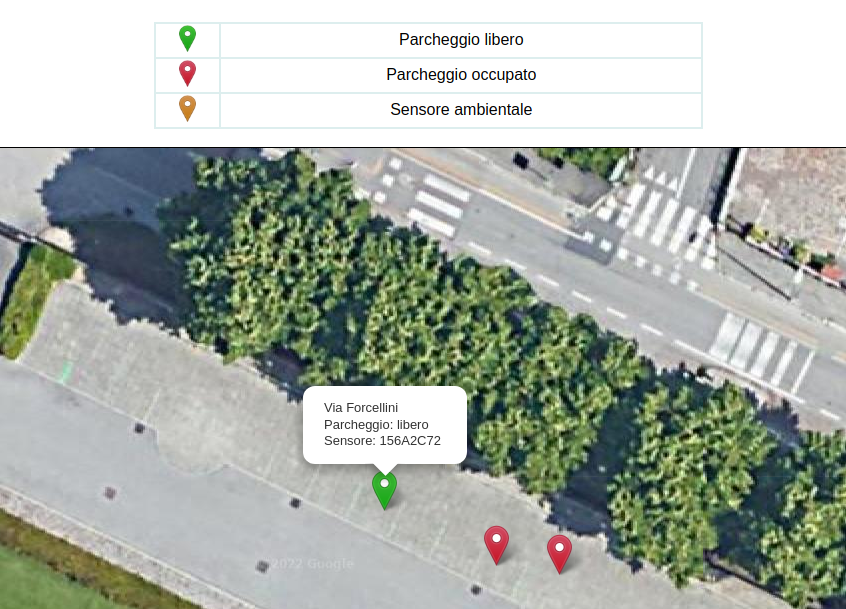
\includegraphics[height=9cm]{front-end-smart-parking}
    \caption{Front-end Smart Parking}
\end{figure}

%**************************************************************
\section{Problematiche riscontrate}
Durante lo svolgimento del progetto si sono presentate alcune criticità, alcune dovute alla mancanza
di conoscenza delle tecnologie da utilizzare. 
\\
Le problematiche riscontrate:

\begin{itemize}
    \item architettura a microservizi: avevo solo una conoscenza basilare
          della tecnologia, grazie al corso d'ingegneria del software ma non
          sufficiente per fare un'analisi di migrazione futura del progetto, in un progetto con 
          architettura a microservizi.
    \item framework Spring: la conoscenza di questo framework era completamente assente
        ed era importante conoscerlo per poter comprendere con chiarezza il software esistente,
        di cui doveva essere effettuata la migrazione.
    \item framework Node.js e NestJS: la conoscenza di questi due framework era completamente
        assente ed era di fondamentale importanza conoscerli per poter implementare il servizio
        di \gls{API} \gls{REST}, lato back-end, richiesto.
    \item La quantità di \gls{API} \gls{REST} da migrare era troppo elevata per il tempo a disposizione.
    \item Il modello della base dati ha dovuto subire adeguamenti rispetto alla prima versione
        per rappresentare nel modo migliore lo scenario funzionale.
\end{itemize}

%**************************************************************
\section{Soluzione scelta}

E' stato scelto di sviluppare il progetto con un architettura di tipo layered architecture. Questo è uno
degli stili architetturali più utilizzati quando si sviluppa un software monolitico. L'idea dietro a 
questa architettura è che i moduli con funzionalità simili sono organizzati in livelli
orizzontali. Quindi ogni livello svolge uno specifico ruolo nell'applicazione.
\\\\
La layered architecture astrae la visione del sistema nel suo insieme, fornendo dettagli 
sufficienti per comprendere ruoli e le responsabilità dei singoli livelli e le relazioni
che intercorrono tra loro.
\\\\
La motivazione che ha portato alla scelta di questo stile architetturale è un'analisi fatta,
che ha rivelato, che la layered si adatta molto bene al servizio di \gls{API} \gls{REST} che
si vuole andare a realizzare. Inoltre molti framework per lo sviluppo di applicativi \gls{back-end} si basano su questo tipo di architettura, tra cui
Spring e NestJS, che sono fondati sul pattern controller-service-repository. Un pattern
che sfrutta la layered architecture, creando tre diversi livelli di astrazione: 
\begin{itemize}
    \item controller: è il livello più alto ed è l'unico responsabile dell'esposizione delle
        funzionalità, in modo che possano essere consumate da entità esterne.
    \item service: livello centrale, gestisce tutta la business logic.
    \item repository: livello più basso, è responsabile di salvare e recuperare i dati da un
        sistema di persistenza, come un database.
\end{itemize}
\leavevmode\newline
Quest'architettura viene utilizzata per effettuare una buona separazione delle responsabilità.
\\
L'architettura usata da Spring e NestJS è proprio la stessa che si è deciso di usare nell'analisi progettuale fatta 
 e quindi questi due framework sono stati scelti per realizzare
la parte di \gls{back-end} del progetto.
\leavevmode\newline
\begin{figure}[H]
    \centering
    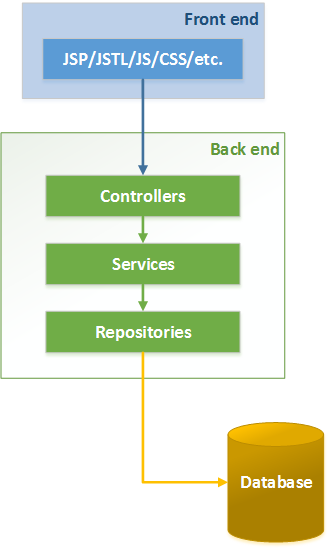
\includegraphics[height=9cm]{controller-service-repository-pattern}
    \caption{Controller-service-repository pattern}
\end{figure}
\leavevmode\newline
Non è prevista la creazione di un sistema di autenticazione per l'uso delle \gls{API} \gls{REST}, in quanto 
un altro studente tirocinante si sta occupando della creazione di questa parte.

%**************************************************************
\section{Descrizione del prodotto ottenuto}

Al momento è disponibile un \gls{back-end} contenente le \gls{API} \gls{REST} sviluppate in NestJS, utilizzabile in produzione,
anche se non potendo migrare l'intero set di \gls{API} \gls{REST} disponibili nella soluzione realizzata in Spring, come preventivato,
sono state sviluppate tutte le \gls{API} \gls{REST} più importanti per effettuare le operazioni \gls{CRUD}\glsfirstoccur più
comuni.
\\\\
Le \gls{API} \gls{REST} espongono un'interfaccia compatibile con quello che ormai è uno standard per la
comunicazione con servizi di tipo \gls{REST}. Ovvero per comunicare con le \gls{API} \gls{REST} bisogna fare
delle richieste \gls{HTTP}\glsfirstoccur a degli specifici \gls{endpoint} con i seguenti metodi \gls{HTTP}:
\begin{itemize}
    \item GET: per ottenere delle risorse dal servizio \gls{REST};
    \item POST: per creare una nuova risorsa nel servizio \gls{REST};
    \item PUT: per modificare una risorsa nel servizio \gls{REST};
    \item DELETE: per eliminare una risorsa dal servizio \gls{REST};
\end{itemize}
\leavevmode\newline
E' presente poi, nel \gls{back-end}, un servizio schedulato che ogni due minuti in maniera autonoma va a fare il polling
da un file \gls{XML}\glsfirstoccur online, contenente gli stati aggiornati dei sensori. Questo servizio registra poi 
le variazioni, rispetto
al polling precedente, nel servizio di persistenza.
\\\\
Il file \gls{XML} viene scritto e gestito dai produttori dei sensori di parcheggio, quindi non è compito di questo 
progetto gestirne il funzionamento. Il funzionamento di questo file \gls{XML} è comunque abbastanza banale,
in quanto ad ogni variazione di stato il sensore di parcheggio va semplicemente ad aggiornare 
il record a lui associato
all'interno del file.
\\\\

%**************************************************************
\section{Tecnologie utilizzate}

\textbf{Git}
\\\\
E' uno degli strumenti di controllo di versionamento più utilizzati. Facilita la collaborazione
tra gli sviluppatori nella realizzazione di un progetto e permette con semplicità di spostarsi
tra varie versioni del software realizzate. Nel progetto è stato utilizzato con il workflow
Gitflow.
\\\\\\
\textbf{Visual Studio Code}
\\\\
E' un editor di codice sorgente sviluppato da Microsoft che aiuta lo sviluppatore durante la fase
di sviluppo del codice in quanto evidenzia le parole chiave, segnala errori di scrittura, suggerisce
snippet di codice. Possiede una grande libreria di estensioni facilmente installabili per renderlo
compatibile con praticamente qualsiasi linguaggio di programmazione.
\\\\\\
\textbf{Postman}
\\\\
E' un'applicazione che viene utilizzata solitamente per testare \gls{API}. E' un client \gls{HTTP} che testa richieste
\gls{HTTP} utilizzando una \gls{GUI}\glsfirstoccur, attraverso la quale otteniamo diversi tipi di risposta in base alle \gls{API} che 
andiamo ad interrogare.
\\\\\\
\textbf{Stoplight}
\\\\
E' una piattaforma per progettare \gls{API}. Grazie a questo strumento è possibile documentare in maniera rigorosa
e su uno spazio in cloud un set di \gls{API}. La piattaforma permette di specificare varie informazioni per ogni
\gls{API}, tra cui \gls{endpoint}\glsfirstoccur, parametri in ingresso attesi, possibili risposte con status code associato. Questo
strumento è molto utile per gli sviluppatori \gls{front-end} che devono chiamare le \gls{API} di un servizio
\gls{back-end}, soprattutto grazie alla funzionalità che permette di generare il \gls{mock}\glsfirstoccur della risposta di un'\gls{API}, 
permettendo allo sviluppatore di effettuare le chiamate al \gls{back-end} anche senza che questo sia stato ancora realizzato.
\\\\\\
\textbf{TypeScript}
\\\\
E' un superset di JavaScript, che aggiunge tipi, classi, interfacce e moduli opzionali al JavaScript 
tradizionale. Si tratta sostanzialmente di una estensione di JavaScript.
TypeScript è un linguaggio tipizzato, ovvero aggiunge definizioni di tipo statico: i tipi consentono di 
descrivere la forma di un oggetto, documentandolo meglio e consentendo a TypeScript di verificare che 
il codice funzioni correttamente.
\\\\\\
\textbf{Node.js}
\\\\
E' un runtime system open source per eseguire applicazioni scritte in JavaScript, permettendoci di utilizzare questo 
linguaggio, tipicamente utilizzato nella client-side, anche per la scrittura di applicazioni server-side.
La piattaforma è basata sul JavaScript Engine V8, che è il runtime di Google utilizzato anche da Chrome e 
disponibile sulle principali piattaforme, anche se maggiormente performante su sistemi operativi UNIX-like.
\\\\\\
\textbf{NestJS}
\\\\
E' un framework per la creazione di applicazioni lato server Node.js efficienti e scalabili. 
Utilizza JavaScript ma è costruito con e supporta completamente TypeScript. Aggiunge un livello di astrazione
al framework Express, che a sua volta aggiunge astrazione al framework Node.js. Di conseguenza NestJS 
utilizza Node.js per eseguire il codice JavaScript generato dalla compilazione del codice TypeScript.
\\\\\\
\textbf{Spring}
\\\\
Spring è un framework leggero, basato su Java. Questo framework integra soluzioni a vari problemi tecnici
che si presentano con alta frequenza durante lo sviluppo software. Spring si basa su due design pattern
fondamentali che sono l'Inversion of Control e Dependency Injection.
\\\\\\
\textbf{PostgreSQL}
\\\\
Chiamato anche Postgres, è un sistema di database relazionale a oggetti (ORDBMS), open source e 
gratuito.
Le principali caratteristiche di Postgres sono affidabilità, integrità dei dati, funzionalità ed estensibilità, 
oltre alla propria community open source che gestisce, aggiorna e sviluppa soluzioni performanti e innovative.
\\\\\\
\textbf{Jest}
\\\\
Jest è un framework di unit test sviluppato da Facebook. Focalizzato sulla semplicità, è utilizzabile in qualsiasi
progetto JavaScript. E'uno dei framework di test JavaScript più popolare in questi giorni e la scelta di default 
per alcuni framework come NestJS e React.
\\\\\\
\textbf{Winston}
\\\\
Winston è una delle libreria più famose per effettuare il logging su applicazioni Node.js. Permette di effettuare il logging
su più livelli di informazione, formattare il logging in modo predefinito, scegliere la destinazione di output del log e molte 
altre opzioni.
\\\\\\
\textbf{Npm}
\\\\
E' uno dei gestori di pacchetti per il linguaggio JavaScript più popolare. E' il gestore di pacchetti predefinito 
per Node.js.

%**************************************************************
\section{Organizzazione del testo}

\begin{description}
    \item[{\hyperref[cap:analisi-requisiti]{Il secondo capitolo}}] descrive l'analisi dei requisiti.
    
    \item[{\hyperref[cap:progettazione]{Il terzo capitolo}}] approfondisce la fase di progettazione.
    
    \item[{\hyperref[cap:ristrutturazione-database]{Il quarto capitolo}}] descrive la fase di ristrutturazione del database.
    
    \item[{\hyperref[cap:verifica-e-validazione]{Il quinto capitolo}}] descrive la fase di verifica e validazione.
    
    \item[{\hyperref[cap:analisi-comparativa]{Il sesto capitolo}}] approfondisce l'analisi comparativa tra la soluzione in Spring e quella in NestJS.
    
    \item[{\hyperref[cap:conclusioni]{Il settimo capitolo}}] presenta le conclusioni finali sul progetto e sull'esperienza di stage.
\end{description}

Riguardo la stesura del testo, relativamente al documento sono state adottate le seguenti convenzioni tipografiche:
\begin{itemize}
	\item gli acronimi, le abbreviazioni e i termini ambigui o di uso non comune menzionati vengono definiti nel glossario, situato alla fine del presente documento;
	\item per la prima occorrenza dei termini riportati nel glossario viene utilizzata la seguente nomenclatura: \emph{parola}\glsfirstoccur;
\end{itemize}             % Introduzione
% !TEX encoding = UTF-8
% !TEX TS-program = pdflatex
% !TEX root = ../tesi.tex

%**************************************************************
\chapter{Analisi dei requisiti}
\label{cap:analisi-requisiti}
%**************************************************************
\intro{In questo capitolo viene descritta la fase di analisi dei requisiti effettuata per
la realizzazione del progetto.}

\section{Scopo del progetto}
Uno sviluppatore prima di me ha realizzato un set di \gls{API} \gls{REST} per gestire le funzionalità del progetto Smart Parking 
e un servizio di polling che va a prendere lo stato dei sensori di parcheggio, aggiornato 
in un file \gls{XML} online e salva le variazioni nel servizio di persistenza.
\\\\
Lo scopo di questo progetto è migrare le \gls{API} \gls{REST} e il servizio di polling, dalla soluzione
realizzata con il framework Spring, in una soluzione realizzata con il framework NestJS.

\section{Confronto con gli stakeholders}
E' stato fatto un incontro iniziale con il proponente, ovvero l'azienda Sync Lab,
per definire con chiarezza i requisiti richiesti.
\subsection{Servizio API REST}
Nell'incontro sono state prese in considerazione le \gls{API} \gls{REST} esistenti (realizzate con il framework Spring) 
di cui doveva essere fatta la migrazione.
E' emerso subito che la quantità di \gls{API} \gls{REST} da realizzare era troppo elevata per il
tempo di stage a disposizione. 
\\\\
E' stato quindi necessario fare una valutazione di quali fossero i servizi fondamentali che
il servizio di \gls{API} \gls{REST} avrebbe dovuto esporre, per poter essere utilizzato senza che venissero
a mancare funzionalità fondamentali per un utilizzo a livello base del sistema.

\subsection{Servizio di polling}
Abbiamo poi valutato il secondo punto importante per questo progetto, ovvero
la necessità di avere le informazioni sullo stato dei sensori sempre aggiornate.
\\\\
La rete dei sensori cresce in maniera dinamica, in quanto un nuovo sensore viene aggiunto/spostato
da un parcheggio senza che un utenza manuale informi il sistema. 
\\
Ma è necessario che quando un sensore si aggiunge alla rete, il sistema lo rilevi e ne mantenga lo stato
aggiornato. La stessa cosa deve avvenire per quanto riguarda lo spostamento di un sensore, solo che in 
questo caso il sistema deve aggiornare le coordinate del sensore esistente, anziché aggiungerne uno nuovo.
\\\\
Sono stati scelti una tipologia di sensori con \gls{GPS}\glsfirstoccur integrato, che ad ogni variazione di stato vanno ad 
aggiornare un record a loro associato in un file \gls{XML} online, dove ogni record contiene le informazioni e
lo stato del sensore.
\\
% //TODO: sistemare grandezza font:
\begin{lstlisting}[style=XML]
<markers>
    <marker id="1" name="156A2C71" address="Padova Galleria Spagna" lat="45.389040" lng="11.928577" state="0" battery="3,7V" active="1"/>
    <marker id="2" name="156A2A71" address="Padova Galleria Spagna" lat="45.389029" lng="11.928598" state="1" battery="3,7V" active="1"/>
    <marker id="3" name="156A2B71" address="Padova Galleria Spagna" lat="45.389028" lng="11.928631" state="0" battery="3,7V" active="1"/>
    <marker id="4" name="156A2C72" address="Via Forcellini" lat="45.392648" lng="11.904846" state="0" battery="3,7V" active="1"/>
    <marker id="5" name="156A2A73" address="Via Forcellini" lat="45.392618" lng="11.904963" state="1" battery="3,7V" active="1"/>
    <marker id="6" name="156A2B74" address="Via Forcellini" lat="45.392622" lng="11.904921" state="1" battery="3,7V" active="1"/>
    <marker id="7" name="156A2C75" address="Piazza Capitaniato" lat="45.407958" lng="11.872594" state="0" battery="3,7V" active="1"/>
    <marker id="8" name="156A2A76" address="Piazza Capitaniato" lat="45.407936" lng="11.872584" state="1" battery="3,7V" active="1"/>
    <marker id="9" name="156A2B77" address="Piazza Capitaniato" lat="45.407913" lng="11.872580" state="0" battery="3,7V" active="1"/>
    <marker id="10" name="156A2C78" address="Prato della valle" lat="45.397848" lng="11.875080" state="1" battery="3,7V" active="1"/>
    <marker id="11" name="156A2A79" address="Prato della valle" lat="45.397838" lng="11.875102" state="0" battery="3,7V" active="1"/>
    <marker id="12" name="156A2B710" address="Prato della valle" lat="45.397822" lng="11.875126" state="0" battery="3,7V" active="1"/>
    <marker id="13" name="156A2C711" address="Via Sorio" lat="45.400546" lng="11.855238" state="0" battery="3,7V" active="1"/>
    <marker id="14" name="156A2A712" address="Via Sorio" lat="45.400547" lng="11.855173" state="0" battery="3,7V" active="1"/>
    <marker id="15" name="156A2B7113" address="Via Sorio" lat="45.400546" lng="11.855015" state="1" battery="3,7V" active="1"/>
</markers>
\end{lstlisting}
\leavevmode\newline
Non avendo controllo sui sensori e quindi su dove vengano scritti i dati, con la proponente si è deciso
di effettuare un polling ogni due minuti al file \gls{XML} e aggiornare lo stato del \gls{back-end}.
\\\\
Lo stato dei sensori è quindi ridondante in quanto è presente sia nel \gls{back-end} del progetto che sul file \gls{XML} online. 
La scelta di duplicare lo stato dei sensori nel \gls{back-end} è stata fatta per trarne i seguenti benefici:
\begin{itemize}
    \item permette di organizzare i dati in maniera più consona e organizzata.
    \item l'accesso ai dati diventa molto più veloce in quanto non si deve interrogare un file \gls{XML} online
        in una posizione remota e sconosciuta ma viene interrogato il servizio di persistenza del \gls{back-end}, 
        di cui abbiamo pieno controllo.
\end{itemize}
\leavevmode\newline
La motivazione che ha portato ad eseguire il polling ogni due minuti è la seguente:
\\
il tipo di servizio offerto non ha bisogno di essere un \gls{real-time system}\glsfirstoccur, in quanto non crea problemi all'utente
vedere una piazzola che si libera/occupa con un delta di intervallo di ritardo. 
\\\\
L'importante è che questo delta non sia troppo elevato, in tal caso i dati mostrati agli utenti sarebbero troppo
inconsistenti per risultare utili. Mentre un delta troppo piccolo genera un carico di lavoro per l'applicazione molto
elevato.
\\\\
Infatti effettuare il polling con un piccolo intervallo di tempo tra un polling e il successivo (dell'ordine dei millisecondi
ad esempio),
genera la produzione di molte 
chiamate \gls{HTTP} da parte del \gls{back-end} per accedere al contenuto del file \gls{XML} e molti accessi al database in caso ci siano dati da 
inserire/aggiornare.
\clearpage
\leavevmode\newline
Vediamo un esempio pratico con una tabella che mostra il costo di chiamate e accessi al database giornalieri al variare 
dell'intervallo di tempo del polling:
% //TODO: aggiungere caption immagini
\renewcommand{\arraystretch}{1.5}
\begin{table}[H]
    \begin{tabular}{|p{2.85cm}|p{3.05cm}|p{3.05cm}|p{3.35cm}|} 
    \hline
    \textbf{Polling} & \textbf{\# chiamate http}  & \textbf{\# accessi lettura} & \textbf{\# accessi scrittura} \\ 
    \hline
    60 minuti & 24 & 24 * $10^3$ & 24 * $10^3$ \\
    \hline
    30 minuti & 48 & 48 * $10^3$ & 48 * $10^3$ \\
    \hline
    15 minuti & 96 & 96 * $10^3$ & 96 * $10^3$ \\
    \hline
    5 minuti & 288 & 288 * $10^3$ & 1440 * $10^2$ \\
    \hline
    2 minuti & 720 & 720 * $10^3$ & 1440 * $10^2$ \\
    \hline
    1 minuto & 1440 & 1440 * $10^3$ & 1440 * $10^2$ \\
    \hline
    1 millisecondo & 864 * $10^5$ & 864 * $10^8$ & 1440 * $10^2$ \\
    \hline
    \end{tabular}
\end{table}
\leavevmode\newline
Per calcolare il numero medio di accessi al database è stata ipotizzata la presenza di 1000 sensori a sistema e che 
ogni cinque minuti la metà dei sensori abbiano bisogno di un aggiornamento (quindi 100 sensori devono essere 
acceduti in scrittura ad ogni minuto). 
\\\\
Quindi si verificano 1000 accessi in lettura ad ogni polling per verificare quali abbiano bisogno di aggiornamento.
Gli accessi in scrittura variano in base al tempo trascorso dall'ultimo polling (da ricordare che gli accessi in scrittura sono molto
più costosi di quelli in lettura).
\\\\
Come vediamo dalla tabella e come auspicabile, con il polling ad un intervallo di ogni ora si effettuano solo
24 richieste \gls{HTTP} al giorno ma il delta di latenza di aggiornamento dei dati ad ogni ora li rende inutilizzabili.
\\\\
D'altra parte un intervallo di un millisecondo rende i dati aggiornati quasi in tempo reale ma 
non è sostenibile effettuare un numero di richieste giornaliere dal \gls{back-end} pari a 864 * $10^5$ (più di 86 milioni).
\leavevmode
\\\\
Un numero di richieste giornaliere pari a 720 è stato ritenuto accettabile, così come il numero di accessi al database
indicati per la colonna dei 2 minuti e si è optato quindi per questa scelta; ritenendo il delta di ritardo di
aggiornamento un valore accettabile per l'utente finale e che i costi delle chiamate e di accessi al database non
siano di sovraccarico per il sistema.
\\\\
Il servizio per il polling dei sensori deve essere realizzato in modo che sia separato da quello delle \gls{API} \gls{REST}.
\\
Sia per una separazione di responsabilità, che per una futura migrazione a un'applicazione basata su microservizi,
in cui il servizio di polling deve diventare un microservizio a se stante, gestibile in maniera indipendente rispetto
agli altri microservizi.

\section{Entità}
Per rendere più chiaro il dominio del progetto ed eliminare eventuali ambiguità, si è ritenuto necessario
documentare le entità di dominio coinvolte nelle funzionalità fondamentali delle \gls{API} \gls{REST}.
\\\\\\
\textbf{Piazzola}
\\\\
Modella il rettangolo bianco dipinto sull'asfalto che delimita la zona in cui l'automobile viene messa
in sosta. Ogni piazzola deve essere associata ad un parcheggio. Una piazzola può avere un solo sensore
di parcheggio.
\\
Ogni piazzola è caratterizzata da:
\begin{itemize}
    \item id: numero incrementale.
    \item latitudine: stringa.
    \item longitudine: stringa.
\end{itemize}
\leavevmode\newline
\textbf{Parcheggio}
\\\\
Modella l'insieme di piazzole.
\\
Ogni parcheggio è caratterizzato da:
\begin{itemize}
    \item id: numero incrementale.
    \item latitudine: stringa.
    \item longitudine: stringa.
\end{itemize}
\leavevmode\newline
\textbf{Sensore}
\\\\
Modella il sensore. Esistono due tipi di sensore:
\begin{itemize}
    \item ambientale: misurana la qualità dell'aria e altri parametri nel parcheggio e possono 
        coprire un'area di N piazzole.
        Sono gestiti da un'altro progetto di tirocinio, quindi non sono facenti parte di questo dominio di progetto.
    \item di parcheggio: sensore posizionato sotto l'auto nella piazzola. Rileva la presenza o meno
        del veicolo. Questo tipo di sensore può essere associato a una sola piazzola.
\end{itemize}
Ogni sensore può avere una sola azienda manutentrice a lui associata.
Ogni sensore è caratterizzato da:
\begin{itemize}
    \item id: numero incrementale.
    \item nome: stringa.
    \item batteria: stringa, indica la tensione della batteria in Volt.
    \item carica: stringa, indica il livello di carica della batteria (da 1 a 3).
    \item type: stringa, indica il tipo di sensore (ambientale o di parcheggio).
    \item attivo: booleano.
    \item ultimo sondaggio: timestamp, indica l'ultima volta che è stato aggiornato lo stato del sensore.
    \item da riparare: booleano, indica se il sensore deve essere riparato.
    \item da caricare: booleano, indica se la batteria del sensore è scarica.
    \item in aggiornamento: booleano, indica se il sensore sta aggiornando il suo software.
\end{itemize}
\leavevmode\newline
\textbf{Manutentore}
\\\\
Modella l'azienda incaricata alla manutenzione dei sensori.
Ogni manutentore è caratterizzato da:
\begin{itemize}
    \item id: numero incrementale.
    \item nome: stringa, indica il nome del titolare dell'azienda.
    \item cognome: stringa, indica il cognome del titolare dell'azienda.
    \item azienda: stringa.
    \item telefono: stringa.
    \item email: stringa.
\end{itemize}
\leavevmode\newline
\textbf{Misurazione sensore parcheggio}
\\\\
Modella la misurazione effettuata dal sensore di parcheggio. A differenza di un sensore ambientale, un sensore
di parcheggio non salva uno storico di misurazioni fatte ma viene inserita solo l'ultima misurazione effettuata,
sovrascrivendo la precedente.
Ogni misurazione di un sensore di parcheggio è caratterizzata da:
\begin{itemize}
    \item id: numero incrementale.
    \item indirizzo: stringa.
    \item latitudine: stringa.
    \item longitudine: stringa.
    \item valore: booleano, indica se il veicolo è presente o meno sopra al sensore.
    \item marca temporale: timestamp, indica la data in cui è stata effettuata la misurazione.
\end{itemize}

\section{Casi d'uso}
Definite le entità di dominio si è proceduto con la creazione dei casi d'uso.
\\
Per maggior chiarezza i casi d'uso sono stati raggruppati per entità di dominio di appartenenza.
\\\\
% parcheggio
\begin{figure}[H]
    \centering
    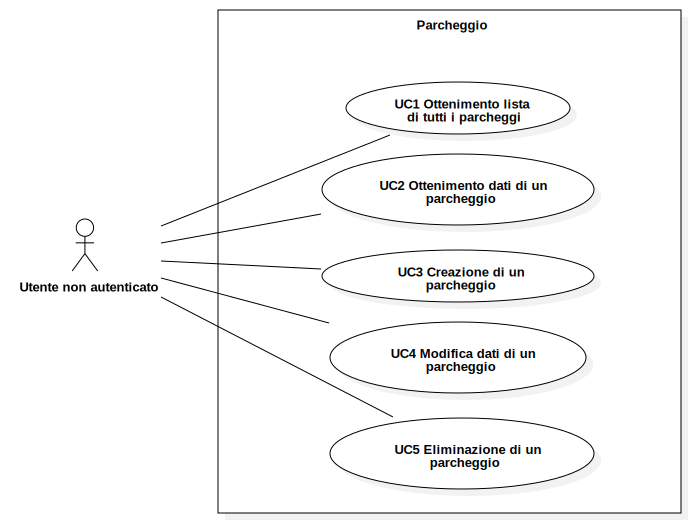
\includegraphics[height=9cm]{usecase/parking-area}
\end{figure}
\leavevmode\newline
\textbf{UC1 - Ottenimento lista di tutti i parcheggi}
\\\\
\textbf{Attori primari:} utente non autenticato.
\\
\textbf{Precondizioni:} l'utente è in possesso degli strumenti per poter effettuare la richiesta al sistema.
\\
\textbf{Post-condizioni:} l'utente ha ottenuto una lista di tutti i parcheggi.
\\
\textbf{Scenario principale:}
\begin{enumerate}
    \item l'utente richiede la lista di tutti i parcheggi.
    \item l'utente ottiene una lista di tutti i parcheggi.
\end{enumerate}
\leavevmode\newline
\textbf{UC2 - Ottenimento dati di un parcheggio}
\\\\
\textbf{Attori primari:} utente non autenticato.
\\
\textbf{Precondizioni:} l'utente è in possesso degli strumenti per poter effettuare la richiesta al sistema.
\\
\textbf{Post-condizioni:} l'utente ha ottenuto i dati di un parcheggio.
\\
\textbf{Scenario principale:}
\begin{enumerate}
    \item l'utente richiede i dati di un parcheggio.
    \item l'utente ottiene i dati di un parcheggio.
\end{enumerate}
\leavevmode\newline
\textbf{UC3 - Creazione di un parcheggio}
\\\\
\textbf{Attori primari:} utente non autenticato.
\\
\textbf{Precondizioni:} l'utente è in possesso degli strumenti per poter effettuare la richiesta al sistema.
\\
\textbf{Post-condizioni:} l'utente ha creato un parcheggio.
\\
\textbf{Scenario principale:}
\begin{enumerate}
    \item l'utente richiede la creazione di un parcheggio.
    \item l'utente crea un parcheggio.
\end{enumerate}
\leavevmode\newline
\textbf{UC4 - Modifica dati di un parcheggio}
\\\\
\textbf{Attori primari:} utente non autenticato.
\\
\textbf{Precondizioni:} l'utente è in possesso degli strumenti per poter effettuare la richiesta al sistema.
\\
\textbf{Post-condizioni:} l'utente ha modificato un parcheggio.
\\
\textbf{Scenario principale:}
\begin{enumerate}
    \item l'utente richiede la modifica di un parcheggio.
    \item l'utente modifica un parcheggio.
\end{enumerate}
\leavevmode\newline
\textbf{UC5 - Eliminazione di un parcheggio}
\\\\
\textbf{Attori primari:} utente non autenticato.
\\
\textbf{Precondizioni:} l'utente è in possesso degli strumenti per poter effettuare la richiesta al sistema.
\\
\textbf{Post-condizioni:} l'utente ha eliminato un parcheggio.
\\
\textbf{Scenario principale:}
\begin{enumerate}
    \item l'utente richiede l'eliminazione di un parcheggio.
    \item l'utente elimina un parcheggio.
\end{enumerate}
\clearpage
% manutentore
\leavevmode\newline

\begin{figure}[H]
    \centering
    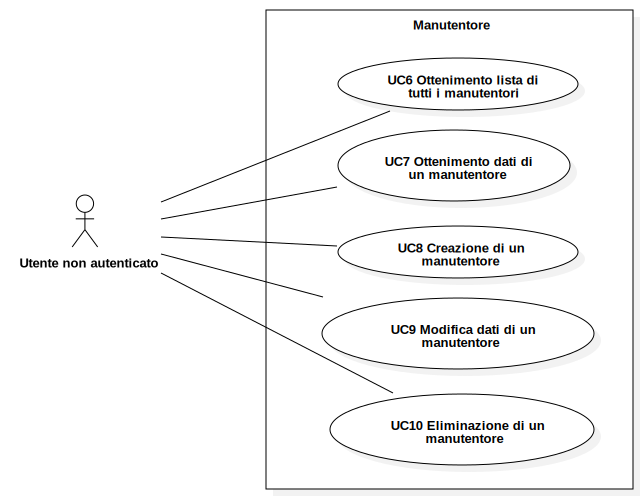
\includegraphics[height=9cm]{usecase/maintainer}
\end{figure}
\textbf{UC6 - Ottenimento lista di tutti i manutentori}
\\\\
\textbf{Attori primari:} utente non autenticato.
\\
\textbf{Precondizioni:} l'utente è in possesso degli strumenti per poter effettuare la richiesta al sistema.
\\
\textbf{Post-condizioni:} l'utente ha ottenuto una lista di tutti i manutentori.
\\
\textbf{Scenario principale:}
\begin{enumerate}
    \item l'utente richiede la lista di tutti i manutentori.
    \item l'utente ottiene una lista di tutti i manutentori.
\end{enumerate}
\leavevmode\newline
\textbf{UC7 - Ottenimento dati di un manutentore}
\\\\
\textbf{Attori primari:} utente non autenticato.
\\
\textbf{Precondizioni:} l'utente è in possesso degli strumenti per poter effettuare la richiesta al sistema.
\\
\textbf{Post-condizioni:} l'utente ha ottenuto i dati di un manutentore.
\\
\textbf{Scenario principale:}
\begin{enumerate}
    \item l'utente richiede i dati di un manutentore.
    \item l'utente ottiene i dati di un manutentore.
\end{enumerate}
\leavevmode\newline
\textbf{UC8 - Creazione di un manutentore}
\\\\
\textbf{Attori primari:} utente non autenticato.
\\
\textbf{Precondizioni:} l'utente è in possesso degli strumenti per poter effettuare la richiesta al sistema.
\\
\textbf{Post-condizioni:} l'utente ha creato un manutentore.
\\
\textbf{Scenario principale:}
\begin{enumerate}
    \item l'utente richiede la creazione di un manutentore.
    \item l'utente crea un manutentore.
\end{enumerate}
\leavevmode\newline
\textbf{UC9 - Modifica dati di un manutentore}
\\\\
\textbf{Attori primari:} utente non autenticato.
\\
\textbf{Precondizioni:} l'utente è in possesso degli strumenti per poter effettuare la richiesta al sistema.
\\
\textbf{Post-condizioni:} l'utente ha modificato un manutentore.
\\
\textbf{Scenario principale:}
\begin{enumerate}
    \item l'utente richiede la modifica di un manutentore.
    \item l'utente modifica un manutentore.
\end{enumerate}
\leavevmode\newline
\textbf{UC10 - Eliminazione di un manutentore}
\\\\
\textbf{Attori primari:} utente non autenticato.
\\
\textbf{Precondizioni:} l'utente è in possesso degli strumenti per poter effettuare la richiesta al sistema.
\\
\textbf{Post-condizioni:} l'utente ha eliminato un manutentore.
\\
\textbf{Scenario principale:}
\begin{enumerate}
    \item l'utente richiede l'eliminazione di un manutentore.
    \item l'utente elimina un manutentore.
\end{enumerate}
\clearpage
% sensore
\leavevmode\newline
\begin{figure}[H]
    \centering
    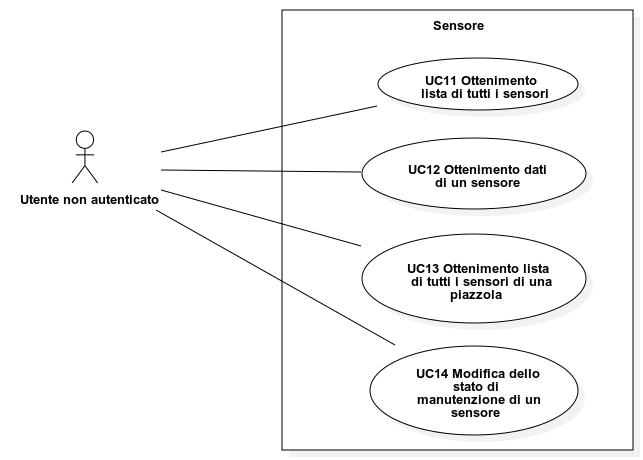
\includegraphics[height=9cm]{usecase/sensor}
\end{figure}
\textbf{UC11 - Ottenimento lista di tutti i sensori}
\\\\
\textbf{Attori primari:} utente non autenticato.
\\
\textbf{Precondizioni:} l'utente è in possesso degli strumenti per poter effettuare la richiesta al sistema.
\\
\textbf{Post-condizioni:} l'utente ha ottenuto una lista di tutti i sensori.
\\
\textbf{Scenario principale:}
\begin{enumerate}
    \item l'utente richiede la lista di tutti i sensori.
    \item l'utente ottiene una lista di tutti i sensori.
\end{enumerate}
\leavevmode\newline
\textbf{UC12 - Ottenimento dati di un sensore}
\\\\
\textbf{Attori primari} utente non autenticato.
\\
\textbf{Precondizioni:} l'utente è in possesso degli strumenti per poter effettuare la richiesta al sistema.
\\
\textbf{Post-condizioni:} l'utente ha ottenuto i dati di un sensore.
\\
\textbf{Scenario principale:}
\begin{enumerate}
    \item l'utente richiede i dati di un sensore.
    \item l'utente ottiene i dati di un sensore.
\end{enumerate}
\leavevmode\newline
\textbf{UC13 - Ottenimento lista di tutti i sensori di una piazzola}
\\\\
\textbf{Attori primari:} utente non autenticato.
\\
\textbf{Precondizioni:} l'utente è in possesso degli strumenti per poter effettuare la richiesta al sistema.
\\
\textbf{Post-condizioni:} l'utente ha ottenuto una lista di tutti i sensori di una piazzola.
\\
\textbf{Scenario principale:}
\begin{enumerate}
    \item l'utente richiede la lista di tutti i sensori di una piazzola.
    \item l'utente ottiene una lista di tutti i sensori di una piazzola.
\end{enumerate}
\leavevmode\newline
\textbf{UC14 - Modifica dello stato di manutenzione di un sensore}
\\\\
\textbf{Attori primari:} utente non autenticato.
\\
\textbf{Precondizioni:} l'utente è in possesso degli strumenti per poter effettuare la richiesta al sistema.
\\
\textbf{Post-condizioni:} l'utente ha modificato lo stato di manutenzione di un sensore.
\\
\textbf{Scenario principale:}
\begin{enumerate}
    \item l'utente richiede la modifica dello stato di manutenzione di un sensore.
    \item l'utente modifica lo stato di manutenzione di un sensore.
\end{enumerate}

% piazzola
\leavevmode\newline
\begin{figure}[H]
    \centering
    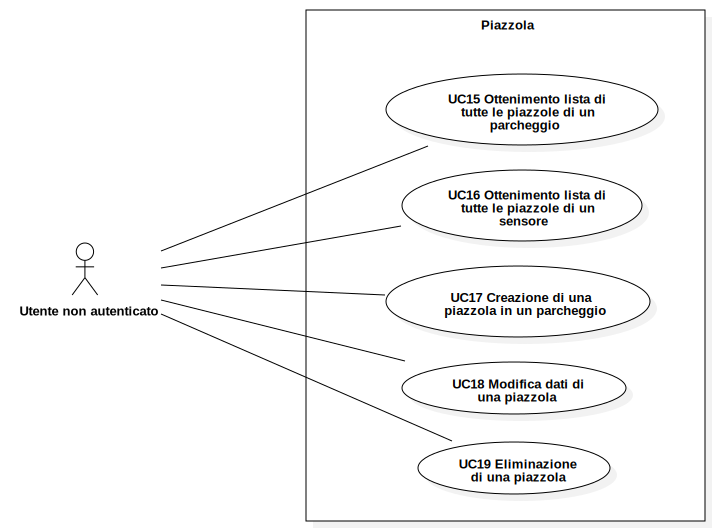
\includegraphics[height=9cm]{usecase/parking-spot}
\end{figure}
\textbf{UC15 - Ottenimento lista di tutte le piazzole di un parcheggio}
\\\\
\textbf{Attori primari:} utente non autenticato.
\\
\textbf{Precondizioni:} l'utente è in possesso degli strumenti per poter effettuare la richiesta al sistema.
\\
\textbf{Post-condizioni:} l'utente ha ottenuto una lista di tutte le piazzole di un parcheggio.
\\
\textbf{Scenario principale:}
\begin{enumerate}
    \item l'utente richiede la lista di tutte le piazzole di un parcheggio.
    \item l'utente ottiene una lista di tutte le piazzole di un parcheggio.
\end{enumerate}
\leavevmode\newline
\textbf{UC16 - Ottenimento lista di tutte le piazzole di un sensore}
\\\\
\textbf{Attori primari:} utente non autenticato.
\\
\textbf{Precondizioni:} l'utente è in possesso degli strumenti per poter effettuare la richiesta al sistema.
\\
\textbf{Post-condizioni:} l'utente ha ottenuto una lista di tutte le piazzole di un sensore.
\\
\textbf{Scenario principale:}
\begin{enumerate}
    \item l'utente richiede la lista di tutte le piazzole di un sensore.
    \item l'utente ottiene una lista di tutte le piazzole di un sensore.
\end{enumerate}
\leavevmode\newline
\textbf{UC17 - Creazione di una piazzola in un parcheggio}
\\\\
\textbf{Attori primari:} utente non autenticato.
\\
\textbf{Precondizioni:} l'utente è in possesso degli strumenti per poter effettuare la richiesta al sistema.
\\
\textbf{Post-condizioni:} l'utente ha creato una piazzola in un parcheggio.
\\
\textbf{Scenario principale:}
\begin{enumerate}
    \item l'utente richiede la creazione di una piazzola in un parcheggio.
    \item l'utente crea una piazzola in un parcheggio.
\end{enumerate}
\leavevmode\newline
\textbf{UC18 - Modifica dati di una piazzola}
\\\\
\textbf{Attori primari:} utente non autenticato.
\\
\textbf{Precondizioni:} l'utente è in possesso degli strumenti per poter effettuare la richiesta al sistema.
\\
\textbf{Post-condizioni:} l'utente ha modificato una piazzola.
\\
\textbf{Scenario principale:}
\begin{enumerate}
    \item l'utente richiede la modifica di una piazzola.
    \item l'utente modifica una piazzola.
\end{enumerate}
\leavevmode\newline
\textbf{UC19 - Eliminazione di una piazzola}
\\\\
\textbf{Attori primari:} utente non autenticato.
\\
\textbf{Precondizioni:} l'utente è in possesso degli strumenti per poter effettuare la richiesta al sistema.
\\
\textbf{Post-condizioni:} l'utente ha eliminato una piazzola.
\\
\textbf{Scenario principale:}
\begin{enumerate}
    \item l'utente richiede l'eliminazione di una piazzola.
    \item l'utente elimina una piazzola.
\end{enumerate}

% misurazione
\leavevmode\newline
\begin{figure}[H]
    \centering
    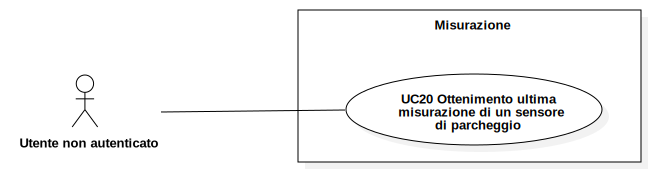
\includegraphics[height=3cm]{usecase/parking-sensor}
\end{figure}
\textbf{UC20 - Ottenimento ultima misurazione di un sensore di parcheggio}
\\\\
\textbf{Attori primari:} utente non autenticato.
\\
\textbf{Precondizioni:} l'utente è in possesso degli strumenti per poter effettuare la richiesta al sistema.
\\
\textbf{Post-condizioni:} l'utente ha ottenuto l'ultima misurazione di un sensore di parcheggio.
\\
\textbf{Scenario principale:}
\begin{enumerate}
    \item l'utente richiede l'ultima misurazione di un sensore di parcheggio.
    \item l'utente ottiene l'ultima misurazione di un sensore di parcheggio.
\end{enumerate}

% polling sensore
\leavevmode\newline
\textbf{UC21 - Ottenimento lista di tutte le piazzole di un parcheggio}
\\\\
\textbf{Attori primari:} utente non autenticato.
\\
\textbf{Precondizioni:} l'utente è in possesso degli strumenti per poter effettuare la richiesta al sistema.
\\
\textbf{Post-condizioni:} l'utente ha ottenuto una lista di tutte le piazzole di un parcheggio.
\\
\textbf{Scenario principale:}
\begin{enumerate}
    \item l'utente richiede la lista di tutte le piazzole di un parcheggio.
    \item l'utente ottiene una lista di tutte le piazzole di un parcheggio.
\end{enumerate}

\section{Tracciamento dei requisiti}
Ogni requisito è identificato da un codice univoco nel seguente formato:
\begin{itemize}
    \item la prima lettera è sempre R, a indicare la parola requisito
    \item la seconda lettera indica il tipo di requisito:
    \begin{itemize}
        \item F per i requisiti funzionali
        \item Q per i requisiti qualitativi
        \item V per i requisiti di vincolo
    \end{itemize}
    \item un numero progressivo che identifica in modo univoco il requisito.
\end{itemize}
Per maggior chiarezza i requisiti sono stati raggruppati per entità di dominio di appartenenza.
% //TODO: inserire casi d'uso sensors-scraping
% //TODO: inserire requisiti funzionali sensors-scraping
% parcheggio
\leavevmode
\begin{table}[H]
    \begin{tabular}{|p{1cm}|p{6cm}|p{1.9cm}|p{1.8cm}|} 
    \hline
    Codice & Descrizione & Rilevanza &  Fonti \\ 
    \hline
    RF1 & L'utente non autenticato deve poter ottenere la lista di tutti i parcheggi. & Obbligatorio & UC1 \\ 
    \hline
    RF2 & L'utente non autenticato deve poter ottenere i dati di un parcheggio. & Obbligatorio & UC2 \\ 
    \hline
    RF3 & L'utente non autenticato deve poter creare un parcheggio. & Obbligatorio & UC3 \\ 
    \hline
    RF4 & L'utente non autenticato deve poter modificare i dati di un parcheggio. & Obbligatorio & UC4 \\
    \hline
    RF5 & L'utente non autenticato deve poter eliminare un parcheggio. & Obbligatorio & UC5 \\ 
    \hline
    \end{tabular}
\end{table}

% manutentore

\begin{table}[H]
    \begin{tabular}{|p{1cm}|p{6cm}|p{1.9cm}|p{1.8cm}|} 
    \hline
    Codice & Descrizione & Rilevanza &  Fonti \\ 
    \hline
    RF6 & L'utente non autenticato deve poter ottenere la lista di tutti i manutentori. & Obbligatorio & UC6 \\ 
    \hline
    RF7 & L'utente non autenticato deve poter ottenere i dati di un manutentore. & Obbligatorio & UC7 \\ 
    \hline
    RF8 & L'utente non autenticato deve poter creare un manutentore. & Obbligatorio & UC8 \\ 
    \hline
    RF9 & L'utente non autenticato deve poter modificare i dati di un manutentore. & Obbligatorio & UC9 \\
    \hline
    RF10 & L'utente non autenticato deve poter eliminare un manutentore. & Obbligatorio & UC10 \\ 
    \hline
    \end{tabular}
\end{table}

% sensore
\begin{table}[H]
    \begin{tabular}{|p{1cm}|p{6cm}|p{1.9cm}|p{1.8cm}|} 
    \hline
    Codice & Descrizione & Rilevanza &  Fonti \\ 
    \hline
    RF11 & L'utente non autenticato deve poter ottenere la lista di tutti i sensori. & Obbligatorio & UC11 \\ 
    \hline
    RF12 & L'utente non autenticato deve poter ottenere i dati di un sensori. & Obbligatorio & UC12 \\ 
    \hline
    RF13 & L'utente non autenticato deve poter ottenere la lista di tutti i sensori di una piazzola. & Obbligatorio & UC13 \\ 
    \hline
    RF14 & L'utente non autenticato deve poter modificare lo stato di manutenzione di un sensore. & Obbligatorio & UC14 \\ 
    \hline
    \end{tabular}
\end{table}
\clearpage
% piazzola
\begin{table}[H]
    \begin{tabular}{|p{1cm}|p{6cm}|p{1.9cm}|p{1.8cm}|} 
    \hline
    Codice & Descrizione & Rilevanza &  Fonti \\ 
    \hline
    RF15 & L'utente non autenticato deve poter ottenere la lista di tutte le piazzole di un parcheggio. & Obbligatorio & UC15 \\ 
    \hline
    RF16 & L'utente non autenticato deve poter ottenere la lista di tutte le piazzole di un sensore. & Obbligatorio & UC16 \\ 
    \hline
    RF17 & L'utente non autenticato deve poter creare una piazzola in un parcheggio. & Obbligatorio & UC17 \\ 
    \hline
    RF18 & L'utente non autenticato deve poter modificare i dati di una piazzola. & Obbligatorio & UC18 \\
    \hline
    RF19 & L'utente non autenticato deve poter eliminare una piazzola. & Obbligatorio & UC19 \\
    \hline
    \end{tabular}
\end{table}

% misurazione
\begin{table}[H]
    \begin{tabular}{|p{1cm}|p{6cm}|p{1.9cm}|p{1.8cm}|} 
    \hline
    Codice & Descrizione & Rilevanza &  Fonti \\ 
    \hline
    RF20 & L'utente non autenticato deve poter ottenere l'ultima misurazione di un sensore di parcheggio. & Obbligatorio & UC20 \\ 
    \hline
    \end{tabular}
\end{table}

% requisiti di qualità
\begin{table}[H]
    \begin{tabular}{|p{1cm}|p{6cm}|p{1.9cm}|p{1.8cm}|} 
    \hline
    Codice & Descrizione & Rilevanza &  Fonti \\ 
    \hline
    RQ1 & Deve essere presente una suite di test automatici per testare la business logic con una copertura a livello branch
        >= 90\%. & Obbligatorio & Capitolato \\ 
    \hline
    RQ2 & Deve essere presente una suite di test automatici per testare la business logic con una copertura a livello linee
        di codice >= 60\%. & Obbligatorio & Capitolato \\ 
    \hline
    RQ3 & Deve essere presente una documentazione che spieghi le scelte progettuali fatte e i motivi che hanno portato ad effettuare
        tali scelte. & Obbligatorio & Capitolato \\ 
    \hline
    \end{tabular}
\end{table}
\clearpage
% requisiti di vincolo
\begin{table}[H]
    \begin{tabular}{|p{1cm}|p{6cm}|p{1.9cm}|p{1.8cm}|} 
    \hline
    Codice & Descrizione & Rilevanza &  Fonti \\ 
    \hline
    RV1 & Utilizzo del framework NestJS per realizzare l'applicazione. & Obbligatorio & Capitolato \\ 
    \hline
    RV2 & Utilizzo di database PostgreSQL. & Desiderabile & Capitolato \\ 
    \hline
    RV3 & Le \gls{API} \gls{REST} devono poter essere chiamate tramite protocollo \gls{HTTP}. & Obbligatorio & Capitolato \\ 
    \hline
    RV4 & La richiesta di ottenimento delle entità, all'applicazione, deve essere fatta tramite metodo GET. & 
        Obbligatorio & Capitolato \\ 
    \hline
    RV5 & La richiesta di inserimento delle entità, all'applicazione, deve essere fatta tramite metodo POST. & 
        Obbligatorio & Capitolato \\ 
    \hline
    RV6 & La richiesta di modifica delle entità, all'applicazione, deve essere fatta tramite metodo PUT. & 
        Obbligatorio & Capitolato \\ 
    \hline
    RV7 & La richiesta di cancellazione delle entità, all'applicazione, deve essere fatta tramite metodo DELETE. & 
        Obbligatorio & Capitolato \\ 
    \hline
    \end{tabular}
\end{table}             % Processi
% !TEX encoding = UTF-8
% !TEX TS-program = pdflatex
% !TEX root = ../tesi.tex

%**************************************************************
\chapter{Progettazione}
\label{cap:progettazione}

\intro{In questo capitolo viene descritta la fase di progettazione effettuata per
la realizzazione del progetto.}

% %**************************************************************
\section{Architettura del progetto}
Le dimensioni di questo progetto allo stato attuale sono contenute, inoltre deve essere fatta un'analisi
comparativa tra la soluzione finale di questo progetto con un progetto già esistente. Per rendere 
l'analisi comparativa più efficace, è stato scelto di usare la stessa architettura dell'altro progetto, 
ovvero la layered architecture.
\\\\
Questo tipo di architettura velocizza la realizzazione del progetto, a discapito della facilità di
manutenzione ma non è un problema essendo il progetto di dimensioni contenute. In caso
il progetto dovesse crescere fino al punto in cui risulti difficile manutenerlo è sempre possibile
migrarlo a un'architettura a microservizi.

% ref: https://cs.uwaterloo.ca/~m2nagapp/courses/CS446/1195/Arch_Design_Activity/Layered.pdf

\subsection{Layered architecture}
La layered architecture è uno degli stili architetturali più utilizzati al giorno d'oggi. L'idea che sta dietro a
questo tipo di architettura è organizzare i moduli o i componenti con funzionalità simili
in livelli orizzontali. Di conseguenza ogni livello svolge un ruolo specifico nell'applicazione.
\\
La layered architecture non ha restrizioni sul numero di strati che l'applicazione può avere, in quanto 
lo scopo è avere livelli che promuovano il concetto di separazione delle responsabilità.

\begin{figure}[H]
    \centering
    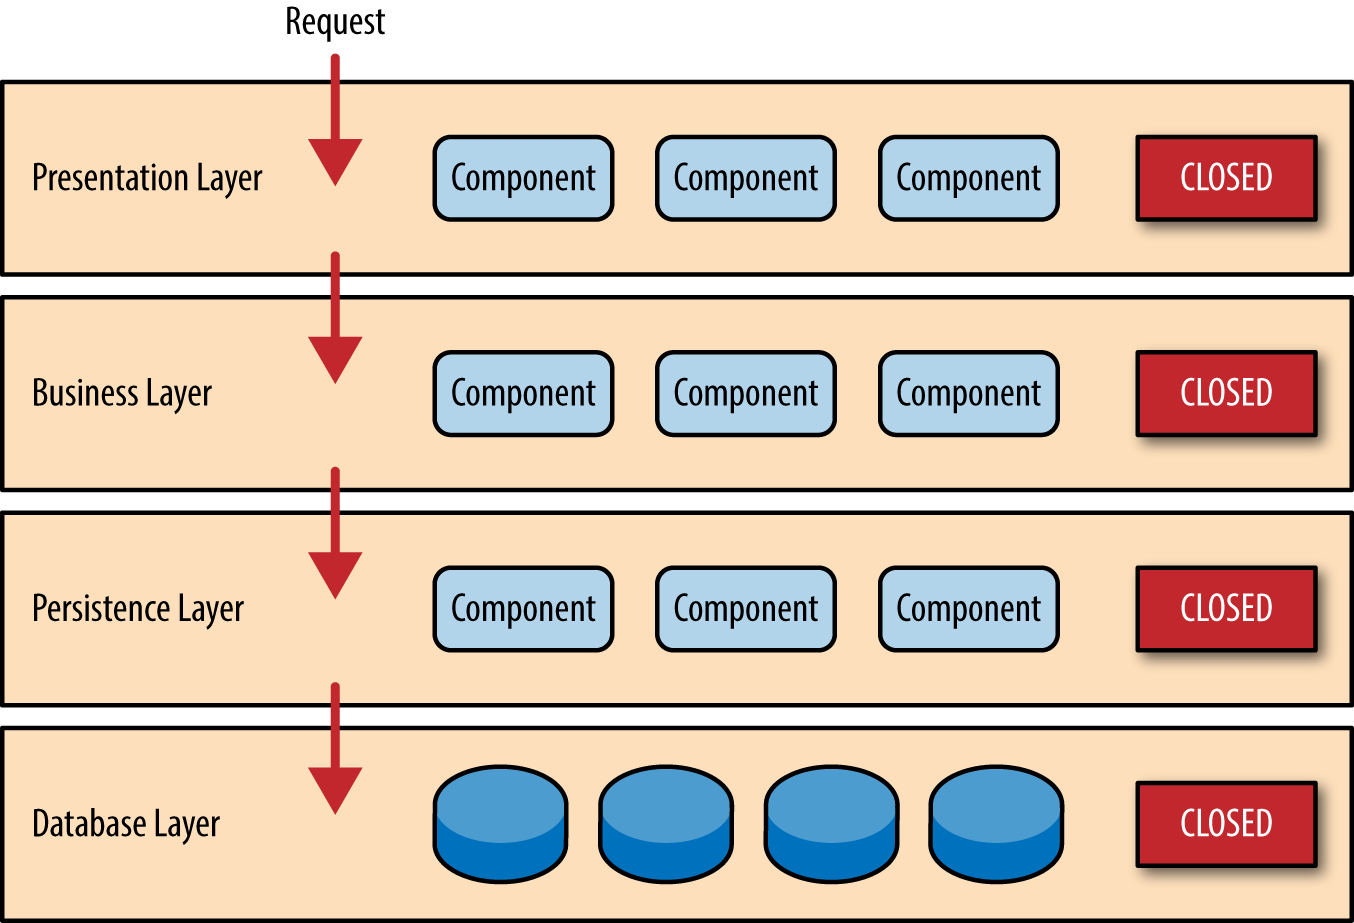
\includegraphics[height=5cm]{layered-architecture}
    \caption{Layered architecture}
\end{figure}
\leavevmode\newline
Solitamente ogni livello comunica solo con il livello sottostante. Il connettore tra ogni livello può 
essere una chiamata di funzione, una richiesta di query, un oggetto dati o qualsiasi connettore che
trasmetta richieste o informazioni.
\\
La denominazione dei livelli è abbastanza flessibile ma di solito sono sempre presenti almeno: un livello di presentazione, un livello
di business e un livello fisico.
\\\\\\
\textbf{Livello di presentazione}
\\\\
Il livello di presentazione contiene tutte le classi responsabili di presentare la visualizzazione delle
delle informazioni all'utente finale. Idealmente questo è il solo livello con cui l'utente finale 
interagisce direttamente.
\\\\\\
\textbf{Livello di business}
\\\\
Il livello di business contiene tutta la logica che è richiesta dall'applicazione per poter soddisfare i 
suoi requisiti funzionali. Solitamente questo livello si occupa dell'aggregazione dei dati, della computazione
e della richiesta dei dati. Quindi qui è dove viene implementata la logica principale dell'applicazione.
\\\\\\
\textbf{Livello fisico}
\\\\
Qui è dove sono salvati tutti i dati recuperabili dell'applicazione. Solitamente questo livello è chiamato
anche livello di persistenza. Questo livello si occupa di interagire con il sistema in cui i dati 
sono mantenuti in maniera persistente, come ad esempio un database.

\subsection{Motivazioni della scelta}
Le motivazione che hanno portato a scegliere questo stile architetturale sono le seguenti:
\begin{itemize}
    \item Dato che la separazione delle responsabilità è la proprietà principale di quest'architettura,
        ogni livello di software ha la sua specifica funzione. Questo rende facile il dover aggiornare 
        singoli livelli e permette al team di sviluppo di separare bene i carichi di lavoro tra i vari 
        membri, che possono lavorare in maniera contemporanea su livelli diversi.
    \item Per la proponente è importante avere una suite di test automatici per testare i vari componenti
        dell'applicazione. La layered architecture separando bene le responsabilità tra i livelli, 
        permette di suddividere l'applicazione in componenti ben separati e quindi più facili da testare.
        Essendo ogni livello isolato dagli altri, è possibile creare casi di test di dimensione ridotta, 
        in quanto le componenti di cui fare il \gls{mock} sono poche.
    \item L'isolamento tra i vari livelli permette di modificare un livello senza che la modifica intacchi
        gli altri livelli.
    \item Nel caso l'applicazione diventi molto grande è possibile, senza troppo sforzo, avviare un processo
        di migrazione ad un'architettura a microservizi. La layered architecture lavora bene (lato monolite) anche
        in un sistema con un'architettura ibrida monolite/microservizi. Questo tipo di architettura
        ibrida solitamente si forma nel processo di migrazione di un sistema monolitico in un sistema a microservizi.
        \\
        Di conseguenza, in ottica di una futura migrazione in un sistema a microservizi (molto probabile che avvenga), è
        bene scegliere un monolite che lavori bene in un'architettura ibrida e quindi che sia facile da migrare
        in un sistema a microservizi.
        \\
        Infatti grazie alla separazione delle responsabilità della layered architecture, è facile andare
        a trasformare i componenti del monolite in microservizi.
\end{itemize}

\section{Struttura software}
E' stato scelto NestJS come framework di sviluppo del progetto dato che utilizza la layered architecture,
tramite il pattern controller-service-repository. Vediamo questo design pattern:
\begin{figure}[H]
    \centering
    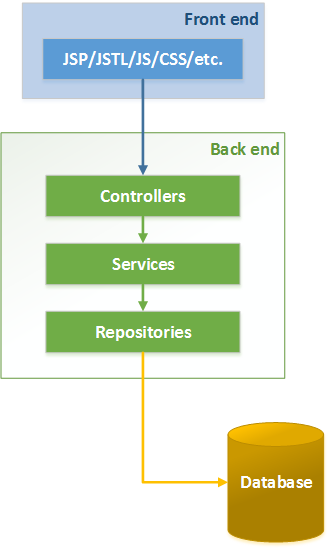
\includegraphics[height=6cm]{controller-service-repository-pattern}
    \caption{Controller-service-repository pattern}
\end{figure}
\leavevmode\newline
Il controller-service-repository pattern suddivide i componenti dell'applicazione su tre livelli fondamentali:
il controller, il service e il repository.
\\
Il controller è il livello più alto, mentre il repository quello più basso, in mezzo ai due c'è il service.
\\
Il controller è il livello responsabile per gestire le richieste in arrivo e ritornare le risposte all'utente finale.
Esiste un meccanismo di routing che gestisce a quale controller inviare le richieste.
\\
Il service è il livello responsabile della business logic.
\\
Il repository è il livello che viene anche chiamato livello di persistenza nella layered architecture e quindi interagisce
con il sistema di persistenza dati, come il database.
\\\\
Analizziamo in dettaglio le componenti che vanno a formare struttura del software:

\subsection{IoC container}
L'Inversion of Control container è un componente fondamentale di NestJS che permette l'applicabilità
del pattern Dependency Injection all'interno di NestJS.
\\
L'IoC container contiene un'istanza di tipo singleton per ogni classe dichiarata come controller o provider.
\\\\
Il funzionamento dell'IoC container è il seguente:
\\\\
quando viene avviata un'applicazione NestJS, il sistema runtime ricerca tutti controller e provider che 
sono stati dichiarati all'interno di moduli importati dal modulo root. Per ognuna di queste classi crea un'istanza
usando il pattern singleton e la inserisce nell'IoC container. 
\\
Se però la classe da istanziare dichiara una dipendenza con un altro controller o provider nel proprio 
costruttore, il sistema runtime applica in maniera automatica il pattern Dependency Injection; ovvero
va a cercare un'istanza della dipendenza dichiarata nel costruttore della classe, nell'IoC container, se
presente la inietta nella classe e crea l'istanza della nuova classe da inserire nell'IoC container. 
\\
Altrimenti va a creare prima
l'istanza della classe che deve essere iniettata, prima della classe che dichiara la dipendenza (se possibile, in quanto la
classe da iniettare potrebbe a sua volta richiedere una dipendenza e in tal caso si segue la successione di 
dipendenze fino a che non si trova una classe che possa essere istanziata) e la inietta nella classe che dichiara
la dipendenza, poi crea un'istanza della classe che ha dichiarato la dipendenza e la inserisce nell'IoC container.

\subsection{Controller e provider}
I due componenti fondamentali di NestJS sono i controller e i provider. 
Per dichiarare una classe come controller, bisogna applicare il decorator @Controller, sopra la 
definizione della classe, mentre per dichiarare una classe come provider bisogna applicare il decorator
@Injectable sopra la definizione della classe.
\\
\begin{lstlisting}[language=JavaScript]
@Injectable()
export class MaintainersRegistryService {
    constructor(private readonly maintainersRegistryRepository: 
        MaintainersRegistryRepository){}

    getAllMaintainers(){
        return this.maintainersRegistryRepository.find();
    }

    async getMaintainerById(id: string){
        const maintainer = 
            await this.maintainersRegistryRepository.findOne({
                where: {
                    id: id
                }
            });

        if(isEmpty(maintainer))
            throw new NotFoundError('maintainer id not found');

        return maintainer;
    }

    async createMaintainer(maintainer: MaintainerRegistry){
        const insertResponse = 
            await this.maintainersRegistryRepository.insert(maintainer);

        if(isEmpty(insertResponse.identifiers))
            throw new InsertError('problem to insert record');

        const maintainerInsertedId = insertResponse.identifiers[0].id;

        return this.getMaintainerById(maintainerInsertedId);
    }

    async editMaintainerById(id: string, maintainerRegistry: MaintainerRegistry){
        try{
            await this.getMaintainerById(id);    
        }catch(error){
            throw(error);
        }
        
        const updateResponse = 
            await this.maintainersRegistryRepository.update(id, maintainerRegistry);

        const numberRowAffected = updateResponse.affected;

        if(numberRowAffected !== 1)
            throw new UpdateError('problem to update record');

        return this.getMaintainerById(id);
    }

    async deleteMaintainerById(id: string){
        try{
            await this.getMaintainerById(id);    
        }catch(error){
            throw(error);
        }

        const deleteResponse = 
            await this.maintainersRegistryRepository.delete(id);

        const numberRowAffected = deleteResponse.affected;

        if(numberRowAffected !== 1)
            throw new DeleteError('problem to delete record');
    }
}
\end{lstlisting}
\leavevmode\newline
\\
I controller sono i componenti dedicati a gestire le richieste in ingresso e a fornire le risposte all'utente
finale. NestJS considera come provider tutte le classi istanziabili e marcate con il decorator 
@Injectable che non sono controller; quindi sia classi di tipo service, che repository devono essere marcate
con il decorator @Injectable. 
\\
\begin{lstlisting}
@Controller('maintainers')
export class MaintainersRegistryController {
    constructor(private readonly maintainersRegistryService: 
        MaintainersRegistryService){}

    @Get()
    getAllMaintainers(){
        return this.maintainersRegistryService
            .getAllMaintainers();
    }

    @Get(':id')
    getMaintainerById(@Param('id') id: string){
        return this.maintainersRegistryService
            .getMaintainerById(id);
    }

    @Post()
    async createMaintainer(@Body() maintainer: MaintainerRegistry){
        return await this.maintainersRegistryService
            .createMaintainer(maintainer);
    }

    @Put(':id')
    editMaintainerById(
        @Param('id') id: string,
        @Body() maintainerRegistry: MaintainerRegistry,
    ){
        return this.maintainersRegistryService
            .editMaintainerById(id, maintainerRegistry);
    }

    @Delete(':id')
    @HttpCode(204)
    deleteMaintainerById(@Param('id') id: string){
        return this.maintainersRegistryService
            .deleteMaintainerById(id);
    }
}
\end{lstlisting}
\leavevmode\newline
\\
E' possibile marcare con il decorator @Injectable
anche classi non service o repository per fare in modo che NestJS, in maniera automatica, istanzi, inietti le dipendenze 
dichiarate nel costruttore e le inserisca nell'IoC container.
\\\\
I controller dell'applicazione individuati sono i seguenti:
\begin{itemize}
    \item MaintainersRegistryController: gestisce le richieste/risposte relative al dominio dei manutentori.
    \item ParkingAreasController: gestisce le richieste/risposte relative al dominio dei parcheggi.
    \item ParkingSensorsController: gestisce le richieste/risposte relative al dominio delle misurazioni
    dei sensori di parcheggio.
    \item ParkingSensorsSensorsController: gestisce le richieste/risposte relative al dominio delle misurazioni
    dei sensori di parcheggio di un sensore.
    \item ParkingSpotsController: gestisce le richieste/risposte relative al dominio delle piazzole.
    \item ParkingSpotsParkingAreasController: gestisce le richieste/risposte relative al dominio delle piazzole
    di un parcheggio.
    \item ParkingSpotsSensorsController: gestisce le richieste/risposte relative al dominio delle piazzole
    di un sensore.
    \item SensorsController: gestisce le richieste/risposte relative al dominio dei sensori.
    \item SensorsParkingSpotsController: gestisce le richieste/risposte relative al dominio dei sensori di una
    piazzola.
    \item SensorsMaintenanceSensorsController: gestisce le richieste/risposte relative al dominio della manutenzione dei
    sensori di un sensore.
\end{itemize}
\leavevmode\newline
I service dell'applicazione individuati sono i seguenti:
\begin{itemize}
    \item MaintainersRegistryService: gestisce la business logic relativa al dominio dei manutentori;
    \item ParkingAreasService: gestisce la business logic relativa al dominio dei parcheggi;
    \item ParkingSensorsService: gestisce la business logic relativa al dominio delle misurazioni dei sensori di parcheggio;
    \item ParkingSpotsService: gestisce la business logic relativa al dominio delle piazzole;
    \item SensorsService: gestisce la business logic relativa al dominio dei sensori;
    \item SensorsMaintenanceService: gestisce la business logic relativa al dominio della manutenzione dei sensori;
    \item SensorsScrapingService: gestisce la business logic relativa al dominio del polling dei sensori;
\end{itemize}
% //TODO: mettere ; alla fine degli itemize
\subsection{Repository}
I repository sono i componenti dedicati alla gestione della persistenza dei dati. Hanno quindi il compito di
comunicare con la componente di archiviazione dati come un database. Nel progetto è stato utilizzato un database
relazionale di tipo postgreSQL.
\\\\
NestJS è indipendente dal tipo di database scelto (relazionale o non relazionale). Infatti NestJS si interfaccia
al database tramite uno strumento che si chiama TypeORM. TypeORM implementa una tecnica di programmazione chiamata 
\gls{ORM}\glsfirstoccur, che converte i dati tra diversi tipi di sistemi usando linguaggi di programmazione \gls{OOP}\glsfirstoccur.
\\\\
Uno strumento \gls{ORM} incapsula il codice necessario per manipolare i dati, senza aver bisogno di scrivere manualmente
le query al database ma si interagisce direttamente con un oggetto nello stesso linguaggio che si sta usando. 
\\
In questo modo il database viene astratto e si diventa indipendenti dal tipo di database utilizzato, in quanto è compito dell'\gls{ORM}
tradurre la richiesta fatta, in linguaggio di programmazione ad alto livello, nella query al database. 
\\\\
Uno strumento come TypeORM offre quindi una grande flessibilità, in quanto è possibile decidere di passare da un database
relazionale a un database non relazionale in qualsiasi momento, senza dover effettuare modifiche al livello di persistenza.
\\\\
Senza un'\gls{ORM} la migrazione da un database relazionale a un database non relazionale implica la riscrittura di tutte le query.
\\\\
Il repository viene fornito e creato in maniera automatica da NestJS. Per fare in modo che ciò avvenga è però necessario
dichiarare, all'interno del modulo in cui si vuole che NestJS crei il repository e in particolare nell'array di imports, con 
il metodo forFeature della classe TypeOrmModule, la lista di entità di cui si vuole creare un repository.
\\\\
Il repository creato da NestJS include tutti i metodi necessari per le operazioni basilari \gls{CRUD} (find(), save(), update(), 
delete() ecc..).
\\\\
Spesso però abbiamo bisogno di effettuare query al database più complesse rispetto a quelle a disposizione nel repository
creato da NestJS. Per fare ciò dobbiamo creare una nostra classe repository custom che estenda la classe Repository, che è una
classe Generic definita all'interno di NestJS e si aspetta come tipo del Generic il tipo dell'entità di cui vogliamo 
creare il repository.
\\\\
Se creiamo un repository custom non è più necessario usare il metodo forFeature nella classe modulo, ma va importato il repository custom
come provider.
\\ 

\begin{lstlisting}
@Injectable()
export class SensorsRepository extends Repository<Sensor>{
    constructor(private dataSource: DataSource){
        super(Sensor, dataSource.createEntityManager());
    }

    getSensorsWithoutSensorMaintenance(){
        return this.dataSource
        .createQueryBuilder()
        .select('sensor')
        .from(Sensor, 'sensor')
        .leftJoin('sensor.sensorMaintenance', 'sensorMaintenance')
        .where('sensorMaintenance.id IS NULL')
        .getMany();
    }
}
\end{lstlisting}
\leavevmode\newline
Nel repository custom, oltre che ai metodi ereditati dalla classe padre Repository, possiamo creare i nostri metodi personalizzati
che eseguono le nostre query custom. 
\\\\
Ci sono 2 modi per creare le query:
\begin{itemize}
    \item tramite notazione pura SQL;
    \item tramite i metodi del Query Builder;
\end{itemize}
\leavevmode\newline
E' fortemente consigliato l'utilizzo del Query Builder anziché usare la notazione SQL pura per 2 motivi:
\begin{enumerate}
    \item La concatenazione dei metodi del Query Builder rende molto più chiaro e pulito il codice, quindi più facile
        da manutenere.
    \item Nel caso di cambio di tipo di database (ad esempio passando da PostgreSQL a Oracle) le query continuano a funzionare, in 
        quanto grazie al Query Builder,
        TypeORM le converte adattandole alla sintassi del database che si stà utilizzando. Mentre non viene 
        effettuata alcun tipo di conversione per le query in notazione pura SQL.
\end{enumerate}
\leavevmode\newline
I repository custom dell'applicazione individuati sono i seguenti:
\begin{itemize}
    \item ParkingSensorsRepository: ha un metodo custom per aggiornare i timestamp delle misurazioni dei sensori di parcheggio 
        passate come parametro.
    \item SensorsRepository: ha un metodo custom per ottenere i sensori che non hanno almeno una manutenzione.
\end{itemize}
% rel: https://it.wikipedia.org/wiki/Object-relational_mapping

\subsection{Moduli}
Un modulo è una componente fondamentale di NestJS. Ogni applicazione ha almeno un modulo, chiamato modulo root. 
Avere solo un modulo non è un caso tipico per un'applicazione, solitamente ce ne sono molti.
I moduli sono utilizzati per organizzare i componenti di un'applicazione.
\\\\
All'interno di uno stesso modulo devono essere presenti componenti appartenenti allo stesso dominio. Ad esempio
il controller, il service e il repository dei sensori di parcheggio sono tre buoni candidati per essere racchiusi 
all'interno dello stesso modulo.
\\\\
Grazie ai moduli si riesce a mantenere il codice ben organizzato, separando le componenti per dominio di appartenenza
e stabilendo dei confini chiari tra i vari componenti. In questo modo NestJS ci aiuta a gestire la complessità e a 
sviluppare con principi SOLID, specialmente quando le dimensioni dell'applicazione crescono e/o quando il team cresce.
\\\\
In un modulo possiamo inserire solo componenti controller o provider. Per inserire un componente in un modulo, dobbiamo
specificare il nome del componente all'interno del decorator
@Module della classe modulo (i controller devono essere dichiarati nell'array controllers di all'interno di @Module,
mentre i provider devono essere dichiarati nell'array providers all'interno di @Module). 
\\\\
Se un controller o un provider non è dichiarato in un modulo che viene incluso dal modulo
root, NestJS non istanzierà la classe del componente e non verrà inserito nell'IoC container.
\\\\
Un concetto fondamentale dei moduli è che le componenti (controller, service, repository, classi varie..) dichiarate 
come appartenenti ad un modulo hanno uno scope locale al modulo, quindi sono visibili solo tra di loro e non vedono
i componenti appartenenti ad altri moduli.
\\
E' un caso comune però che un componente di un modulo abbia bisogno di un componente appartenente ad un altro modulo
e quindi lo dichiara come dipendenza. Facendo una cosa del genere NestJS genera un errore in fase di compilazione, poiché come 
spiegato sopra, un componente di un modulo A, non può vedere un componente di un modulo B.
\\\\
Per risolvere questo problema NestJS permette di definire nel decorator @Module della classe modulo, i componenti che
quel modulo vuole esportare e quindi che abbiano visibilità pubblica (i componenti da esportare devono essere dichiarati 
nell'array exports all'interno di @Module). 
\\
In questo caso se un componente di un modulo B dichiara una 
dipendenza da un componente esportato da un modulo A, nel decorator @Module, della classe modulo B, deve essere dichiarato il
modulo del componente che si vuole importare (i moduli da importare devono essere dichiarati nell'array imports all'interno di @Module).
\\
% //TODO: sistemare colori codice
\begin{lstlisting}
@Module({
    imports: [ 
        SensorsModule,
    ],
    controllers: [
        ParkingSpotsController, 
        ParkingSpotsParkingAreasController,
        ParkingSpotsSensorsController,
    ],
    providers: [
        ParkingSpotsService,
        ParkingSpotsRepository,
    ],
    exports: [
        ParkingSpotsService,
    ],
})
export class ParkingSpotsModule {}
\end{lstlisting}
\leavevmode\newline
I moduli dell'applicazione individuati sono i seguenti:
\begin{itemize}
    \item AutomapperCustomModule: contiene i componenti per effettuare il mappaggio da DTO a entità.
    \item DtoValidatorModule: contiene i componenti per validare i campi di un DTO.
    \item MaintainersRegistryModule: contiene i componenti appartenenti al dominio dei manutentori.
    \item ParkingAreasModule: contiene i componenti appartenenti al dominio dei parcheggi.
    \item ParkingSensorsModule: contiene i componenti appartenenti al dominio delle misurazioni dei sensori di parcheggio.
    \item ParkingSpotsModule: contiene i componenti appartenenti al dominio delle piazzole.
    \item SensorsModule: contiene i componenti appartenenti al dominio dei sensori.
    \item SensorsMaintenanceModule: contiene i componenti appartenenti al dominio della manutenzione dei sensori.
    \item SensorsScrapingModule: contiene i componenti appartenenti al dominio del polling dei sensori.
\end{itemize}

\subsection{DTO}
E' stata usata una classe di tipo \gls{DTO}\glsfirstoccur chiamata SensorsScrapingDto. Questa classe viene utilizzata per rappresentare
il contenuto del file \gls{XML} online contente lo stato dei sensori. Da questo oggetto vengono estratte le informazioni
utili per rappresentare le entità di tipo sensore e misurazioni sensore con cui si va ad aggiornare il database.
\\\\
Prima di effettuare la conversione da \gls{DTO} a entità, i campi del \gls{DTO} vengono validati, lanciando un'eccezione nel caso 
la validazione fallisca.
\\
\begin{lstlisting}
export class SensorScrapingDto{
    
    id: string;

    name: string;

    address: string;

    lat: string;

    lng: string;

    state: boolean;

    battery: string;

    active: boolean;

    constructor(){
        this.id = '0';
        this.name = '';
        this.address = '';
        this.lat = '0';
        this.lng = '0';
        this.state = false;
        this.battery = '';
        this.active = false;
    }
}
\end{lstlisting}
% //TODO: mettere in corsivo parole collegate a elementi del codice
\subsection{Eccezioni}
NestJS ha un livello built-in che è responsabile di processare tutte le eccezioni non catturate durante 
l'esecuzione di un'applicazione.
\\\\
Quando un'eccezione non viene catturata dal codice dell'applicazione, viene catturata da questo livello,
che in maniera automatica invia una risposta user-friendly \gls{HTTP} al client, evitando di far interrompere 
l'esecuzione del programma. Questa componente si chiama exception filter.
\\\\
La risposta inviata al client dall'exception filter è user-friendly e contiene un messaggio appropriato, solo se l'eccezione è di tipo HttpException o 
una sua sottoclasse. 
Altrimenti viene inviata una risposta al client con un messaggio "internal server error" e status code 500.
\\\\
Possono capitare eccezioni anche durante l'esecuzione di query tramite TypeORM. Essendo TypeORM una libreria
esterna, nessuna eccezione da lei lanciata viene catturata dal livello descritto sopra di NestJS.
\\\\
Per evitare di interrompere l'esecuzione del programma al lancio di eccezioni non catturabili dall'exception filter di NestJS,
 si è deciso di 
sovrascrivere l'exception filter globale fornito da NestJS con uno custom e di creare un set di eccezioni
custom che vengono lanciate per problemi collegati al servizio di persistenza.
\\\\
Questo exception filter è stato chiamato TypeOrmExceptionFilter e implementa l'interfaccia ExceptionFilter di
NestJS. 
\\
TypeOrmExceptionFilter simula il comportamento dell'exception filter di NestJS catturando qualsiasi
tipo di eccezione, rispondendo con "internal server error" e status code 500 in caso l'eccezione non sia riconosciuta.
Inoltre funziona anche se si verificano eccezioni da librerie esterne; garantendo un buon livello di resilienza
del programma. 
\\\\
Se l'eccezione lanciata è quella custom, definita per i problemi del servizio di persistenza, lo status code e il messaggio 
vengono inviati in maniera
appropriata all'utente finale.
\\\\
Eccezioni di TypeORM di tipo QueryFailedError, vengono analizzate in base al loro codice di errore; 
lo status code e il messaggio anche in questo caso vengono inviati in maniera appropriata all'utente finale.
Un esempio di eccezione di tipo QueryFailedError con codice errore 23505, indica un confitto nel database, quindi
viene inviata una risposta al client con status code 409 e messaggio "database error on unique constraint".
\\\\
Avere un exception filter permette di spostare la responsabilità della gestione delle eccezioni in un livello
apposito. In questo modo si facilita la manutenzione e si assicura coerenza nella gestione delle eccezioni.
\\\\
Senza un exception filter dovrebbero essere i controller a gestire le eccezioni e modificare la loro risposta
in base al tipo di eccezione ricevuta dal service (che ha usufruito del metodo del repository che ha lanciato
l'eccezione).
\\\\
In questo modo però si creano controller di grandi dimensioni rendendo il codice meno pulito e più difficile
da manutenere. Inoltre questo approccio non garantisce che tutti i controller gestiscano la stessa eccezione
allo stesso modo. 
\\
Ad esempio sviluppatori diversi potrebbero gestire in maniera diversa la stessa eccezione (ad esempio rispondendo
all'utente finale con un messaggio di errore diverso,
più messaggi di errore, inserendo un numero e tipo di parametri di risposta diversi ecc..)
generando confusione per l'utente finale.
\\\\
Le eccezioni custom per TypeORM individuate sono le seguenti:
\begin{itemize}
    \item NotFoundError: gestisce errori dovuti alla richiesta di dati inesistenti.
    \item InsertError: gestisce errori dovuti all'inserimento di dati.
    \item UpdateError: gestisce errori dovuti all'aggiornamento di dati.
    \item DeleteError: gestisce errori dovuti alla cancellazione di dati.
\end{itemize}
\leavevmode\newline

\subsection{Scheduler}
Come spiegato nel capitolo di analisi dei requisiti, si è deciso di implementare il servizio di polling dei dati
dei sensori con un intervallo di tempo pari a due minuti. Per fare questa cosa utilizzo 
la libreria @nestjs/schedule che integra il package cron di Node.js.
\\\\
Questa libreria mette a disposizione uno strumento per poter eseguire il metodo
di una classe ad intervalli di tempo regolari.
\\\\
Per poter usare la libreria bisogna importare, nel modulo root dell'applicazione, il modulo della libreria schedule in questo modo:
\begin{lstlisting}
@Module({
  imports: [
    ScheduleModule.forRoot()
  ],
})
export class AppModule {}
\end{lstlisting}
\leavevmode\newline
Avendo importato la libreria abbiamo a disposizione un decorator @Cron, da specificare sopra al metodo che vogliamo venga 
schedulato. 
\\\\
Come parametro del @Cron dobbiamo inserire una stringa contenente un cron pattern, con
l'intervallo di tempo con cui vogliamo che NestJS esegua il metodo.
\\\\
Nel nostro caso vogliamo eseguirlo ogni due minuti, quindi gli passiamo la stringa "*/2 * * * *".
\\\\
In particolare, il metodo da schedulare è il metodo all'interno del service SensorsScrapingService, che si occupa
di effettuare il polling, la persistenza dei dati dei sensori di parcheggio e delle misurazioni dei sensori di parcheggio.

\subsection{Logging}
Il logging in un'applicazione è un processo fondamentale, che serve a salvare gli eventi che accadono durante
la sua esecuzione.
\\\\
Grazie al logging, gli sviluppatori possono accorgersi di potenziali attacchi o analizzare gli
errori prima che questi interrompano i flussi di lavoro aziendali.
\\\\
Il logging viene effettuato salvando su un file (solitamente con estensione .log) le informazioni rilevanti
accadute in un particolare evento che si è deciso di loggare, come la richiesta da parte
dell'utente finale di un servizio dell'applicazione.
\\\\
Solitamente questi file di log raggiungono dimensioni importanti a volte nell'ordine dei Gigabyte, quindi possono aver bisogno di
un server dedicato per persisterli oppure di meccanismi di compressione file schedulati.
\\\\
Per questo progetto è stato deciso di fare il logging di tutte le richieste alle \gls{API} \gls{REST} da parte dell'utente
finale e tutte le volte che viene eseguito il servizio di polling schedulato.
\\
In particolare, per le richieste alle \gls{API} \gls{REST} dell'utente finale, si vuole effettuare il logging delle seguenti 
informazioni:
\begin{itemize}
    \item metodo della richiesta (GET, POST, PUT, DELETE);
    \item \gls{endpoint} richiesto;
    \item corpo della richiesta;
    \item user agent dell'utente finale;
    \item ip dell'utente finale;
    \item status code di risposta;
    \item lunghezza del messaggio di risposta;
    \item timestamp della richiesta;
\end{itemize}
\leavevmode\newline
Per il servizio di polling si vuole effettuare il logging delle seguenti informazioni:
\begin{itemize}
    \item timestamp del momento di avvio del polling;
    \item timestamp del momento di fine del polling;
\end{itemize}
\leavevmode\newline
NestJS ha una classe built-in, chiamata Logger, che è possibile usare per effettuare il logging 
dell'applicazione. 
\\\\
Questa classe però permette solo di effettuare operazioni basilari e come spiegato nella 
guida ufficiale, per effettuare operazioni più complesse, come il salvataggio delle informazioni di 
logging su file, è bene appoggiarsi ad una libreria esterna che si integra molto bene con NestJS, chiamata
Winston.
\\\\
Con Winston è possibile definire la destinazione di output dei nostri log (nel nostro caso un file .log in una directory logs nel
progetto) e la formattazione nel testo (nel nostro caso abbiamo usato una funzionalità di Winston che permette
di usare la stessa formattazione dei log di NestJS).
\\\\
Le informazioni di cui si può effettuare il logging tramite Winston, assumono diversi livelli. Il livello del log 
indica la sua importanza:
\begin{itemize}
    \item error: log critico, qualcosa nell'applicazione non ha funzionato correttamente e
        alcune funzionalità dell'applicazione potrebbero non funzionare correttamente;
    \item warn: log di avviso, qualcosa di inaspettato è successo nell'applicazione;
    \item info: log di informazione, è successo un evento all'interno dell'applicazione;
\end{itemize}
\leavevmode\newline
Esistono poi altri livelli di log che non sono stati però usati in questo progetto, quindi si è deciso di non specificarli.
\\\\
Winston permette di scegliere quali sono i livelli di informazione che vogliamo loggare, per questo progetto è stato effettuato il logging
a livello error e info.
\\\\
Le informazioni riguardanti le richieste dell'utente finale e il servizio di polling, sono stati loggate a livello info.
\\\\
Per loggare le richieste dell'utente finale è stato implementato un middleware LoggerMiddleware che intercetta tutte le 
richieste dell'utente finale prima che 
vengano passate ai controller e salva in delle variabili interne le informazioni sulla richiesta.
\\\\
Per avere nel log, anche lo status code della risposta inviata all'utente finale dal controller, il LoggerMiddleware imposta un 
listener sull'evento close dell'oggetto response. In questo modo il log viene scritto solo quando il controller ha terminato di
gestire la richiesta e abbiamo tutti i dati a disposizione per poterla loggare.
% ref: https://www.loggly.com/use-cases/application-logging-best-practices/

\begin{lstlisting}
@Injectable()
export class LoggerMiddleware implements NestMiddleware {
  constructor(
    @Inject(WINSTON_MODULE_PROVIDER)
      private readonly logger: Logger
  ){}

  use(request: Request, response: Response, next: NextFunction): void {
    const { ip, method, originalUrl: url } = request;
    const userAgent = request.get('user-agent') || '';
    const body = JSON.stringify(request.body);

    response.on('close', () => {
      const { statusCode } = response;
      const contentLength = response.get('content-length');

      this.logger.info(
        `${method} ${url} ${body} ${statusCode} ${contentLength} - ${userAgent} ${ip}`
      );
    });

    next();
  }
}
\end{lstlisting}

\section{Servizio di polling}
Sono state proposte due varianti per sviluppare il servizio di polling. Queste due varianti riguardano il
modo in cui il servizio SensorsScrapingService, che si occupa di effettuare il polling dei dati dei sensori
da un file \gls{XML} online, debba comunicare col servizio di persistenza.
\\\\
Le due varianti:
\begin{enumerate}
    \item Far comunicare il SensorsScrapingService col servizio di persistenza effettuando delle chiamate \gls{HTTP} 
        alle \gls{API} \gls{REST} di cui ha bisogno.
    \item Far comunicare il SensorsScrapingService direttamente col livello di servizio dei sensori e delle misurazioni 
    dei sensori di parcheggio.
\end{enumerate}
\leavevmode\newline
E' stato scelto di implementare il punto 2. Vediamo le motivazioni che hanno portato a effettuare questa scelta, analizzando pro e 
contro dei due rispettivi punti.
\\\\
Pro del punto 1
\begin{itemize}
    \item Far comunicare il SensorsScrapingService con un servizio di \gls{API} \gls{REST}, separa bene le responsabilità e 
        nel caso di migrazione a un applicazione basata su microservizi, il microservizio dedicato al polling dei sensori 
        non deve cambiare il modo in cui interagisce
        con il servizio di persistenza, in quanto continua a chiamare le stesse \gls{API} \gls{REST} tramite il protocollo \gls{HTTP}.
\end{itemize}
\leavevmode\newline
Contro del punto 1
\begin{itemize}
    \item Come analizzato nella fase di analisi dei requisiti il SensorsScrapingService deve effettuare 720 chiamate \gls{HTTP} giornaliere
        per scaricare i dati dei sensori aggiornati. 
        \\
        Quindi come minimo deve effettuare 720 chiamate \gls{HTTP} giornaliere anche alle \gls{API} \gls{REST}, per verificare se ci sono sensori
        da aggiornare. 
        \\
        Nella pratica le chiamate \gls{HTTP} da fare sono di più, poiché dopo aver verificato se ci sono sensori da aggiornare ed
        eventualmente aggiornati, bisogna fare un'altra chiamata \gls{HTTP} alle \gls{API} \gls{REST} per verificare se ci sono anche misurazioni dei sensori
        da aggiornare ed eventualmente aggiornarle. 
        \\
        Il che porta il numero di chiamate \gls{HTTP} da effettuare al servizio di \gls{API} \gls{REST}, pari ad un minimo di 1440 giornaliere.
\end{itemize}
\leavevmode\newline
Pro del punto 2
\begin{itemize}
    \item Far comunicare direttamente il SensorsScrapingService con il servizio dei sensori e delle misurazioni dei sensori di parcheggio
        riduce notevolmente i costi in termini di carico dell'applicazione, in quanto per persistere i dati è sufficiente chiamare un
        metodo del servizio da cui si dipende, senza dover fare chiamate \gls{HTTP} che sono molto costose. 
\end{itemize}
\leavevmode\newline
Contro del punto 2
\begin{itemize}
    \item Nel caso di migrazione a un'applicazione basata su microservizi bisogna modificare il modo in cui il SensorsScrapingService 
        persiste i dati dei sensori
        e delle misurazioni dei sensori di parcheggio. Probabilmente bisogna passare a effettuare chiamate \gls{HTTP} al servizio di \gls{API} \gls{REST} (come il punto 1),
        in quanto il servizio di polling diventerà un microservizio indipendente, quindi non saranno più a lui visibili il servizio dei 
        sensori e delle misurazioni di parcheggio.
    \item Solitamente è meglio evitare di creare dipendenze tra servizi, per mantenere il servizio il più isolato possibile per il
        concetto di separazione delle responsabilità.
\end{itemize}
\leavevmode\newline
Si è optato per il punto 2, in quanto questo è un progetto nato con lo scopo di fare un'analisi comparativa con un altro progetto esistente
e quindi per non avere differenze prestazionali si è implementato il servizio usando la variante più simile al modo in cui il 
servizio di polling è implementato nell'altro progetto. Inoltre è vero che è bene evitare le dipendenze tra servizi per ridurre
l'accoppiamento tra le componenti e separare le responsabilità ma molto spesso non è possibile farlo e capita frequentemente
di avere dipendenze tra loro.

\section{API REST}
Tramite lo strumento Stoplight sono state progettate 17 \gls{API} \gls{REST}. Stoplight light è un ottimo strumento realizzato
appositamente per progettare \gls{API} \gls{REST}.
\\\\
Essendo un servizio in cloud è accessibile a chiunque abbia necessità di avere la documentazione delle \gls{API} da utilizzare.
\\\\
Stoplight permette di definire l'specificare dell'\gls{API}, il metodo della richiesta per accedere alla risorsa (GET, POST, PUT, DELETE ecc..),
eventuale corpo della richiesta, eventuale corpo della risposta, status code della risposta e altre informazioni
utili a chi deve sviluppare le \gls{API} o all'utente finale che deve effettuare le richieste.
\\\\
Progettata un'\gls{API} su Stoplight è possibile generare il \gls{mock} della risposta, in questo modo gli sviluppatori \gls{front-end} non hanno bisogno
di attendere che il \gls{back-end} venga realizzato per sviluppare la parte di \gls{front-end}.
\\\\
Le \gls{API} \gls{REST}, suddivise per dominio di appartenenza, sono le seguenti:
\\\\
\textbf{Parcheggio}
\\
\begin{table}[H]
    \begin{tabular}{|p{3.2cm}|p{1.4cm}|p{1.4cm}|p{5.8cm}|} 
    \hline
    \textbf{Endpoint} & \textbf{Metodo} & \textbf{Codice risposta} & \textbf{Descrizione} \\ 
    \hline
    /parking-areas & GET & 200 & Restituisce tutti i parcheggi \\ 
    \hline
    /parking-areas & POST & 201 & Crea un parcheggio \\ 
    \hline
    /parking-areas/\{id\} & GET & 200 & Restituisce il parcheggio con l'id richiesto \\ 
    \hline
    /parking-areas/\{id\} & PUT & 200 & Modifica il parcheggio con l'id richiesto \\ 
    \hline
    /parking-areas/\{id\} & DELETE & 204 & Elimina il parcheggio con l'id richiesto \\ 
    \hline
    \end{tabular}
    \caption{API REST parcheggio}
\end{table}
\clearpage
\leavevmode\newline
\textbf{Manutentore}
\\
\begin{table}[H]
    \begin{tabular}{|p{3.2cm}|p{1.4cm}|p{1.4cm}|p{5.8cm}|} 
    \hline
    \textbf{Endpoint} & \textbf{Metodo} & \textbf{Codice risposta} & \textbf{Descrizione} \\ 
    \hline
    /maintainers & GET & 200 & Restituisce tutti i manutentori \\ 
    \hline
    /maintainers & POST & 201 & Crea un manutentore \\ 
    \hline
    /maintainers/\{id\} & GET & 200 & Restituisce il manutentore con l'id richiesto \\ 
    \hline
    /maintainers/\{id\} & PUT & 200 & Modifica il manutentore con l'id richiesto \\ 
    \hline
    /maintainers/\{id\} & DELETE & 204 & Elimina il manutentore con l'id richiesto \\ 
    \hline
    \end{tabular}
    \caption{API REST manutentore}
\end{table}
\leavevmode\newline
\textbf{Sensore}
\\
\begin{table}[H]
    \begin{tabular}{|p{3.2cm}|p{1.4cm}|p{1.4cm}|p{5.8cm}|} 
    \hline
    \textbf{Endpoint} & \textbf{Metodo} & \textbf{Codice risposta} & \textbf{Descrizione} \\ 
    \hline
    /sensors & GET & 200 & Restituisce tutti i sensori \\ 
    \hline
    /sensors/\{id\} & GET & 200 & Restituisce il sensore con l'id richiesto \\ 
    \hline
    /sensors/sensors-maintenance & GET & 200 & Restituisce tutti i sensori con le loro informazioni sulla 
        manutenzione \\ 
    \hline
    /sensors/\{id\}/sensors-maintenance & GET & 200 & Restituisce il sensore con l'id richiesto con le sue 
        informazioni sulla manutenzione \\ 
    \hline
    /sensors/\{id\}/sensors-maintenance & PUT & 200 & Modifica le informazioni di manutenzione del sensore con
        l'id richiesto \\ 
    \hline
    /parking-spots/\{id\}/sensors & GET & 200 & Restituisce tutti i sensori della piazzola con l'id richiesto \\ 
    \hline
    \end{tabular}
    \caption{API REST sensore}
\end{table}
\leavevmode\newline
\textbf{Piazzola}
\\
\begin{table}[H]
    \begin{tabular}{|p{3.2cm}|p{1.4cm}|p{1.4cm}|p{5.8cm}|} 
    \hline
    \textbf{Endpoint} & \textbf{Metodo} & \textbf{Codice risposta} & \textbf{Descrizione} \\ 
    \hline
    /parking-areas/\{id\}/parking-spots & GET & 200 & Restituisce tutte le piazzole del parcheggio con l'id 
    richiesto \\ 
    \hline
    /parking-areas/\{id\}/parking-spots & POST & 201 & Crea una piazzola associata al parcheggio con l'id 
    richiesto \\ 
    \hline
    /parking-spots/\{id\} & PUT & 200 & Modifica la piazzola con l'id richiesto \\ 
    \hline
    /parking-spots/\{id\} & DELETE & 200 & Elimina la piazzola con l'id richiesto \\ 
    \hline
    /sensors/\{id\}/parking-spots & GET & 200 & Restituisce tutte le piazzole del sensore con l'id 
    richiesto \\ 
    \hline
    \end{tabular}
    \caption{API REST piazzola}
\end{table}
\clearpage
\leavevmode\newline
\textbf{Misurazione sensore di parcheggio}
\\
\begin{table}[H]
    \begin{tabular}{|p{3.2cm}|p{1.4cm}|p{1.4cm}|p{5.8cm}|} 
    \hline
    \textbf{Endpoint} & \textbf{Metodo} & \textbf{Codice risposta} & \textbf{Descrizione} \\ 
    \hline
    /sensors/{id}/parking-sensors & GET & 200 & Restituisce tutte le misurazioni del sensore di parcheggio con l'id 
    richiesto (ogni sensore di parcheggio ha solo una misurazione: l'ultima effettuata) \\ 
    \hline
    \end{tabular}
    \caption{API REST misurazione sensore di parcheggio}
\end{table}             % Kick-Off
% !TEX encoding = UTF-8
% !TEX TS-program = pdflatex
% !TEX root = ../tesi.tex

%**************************************************************
\chapter{Analisi dei requisiti}
\label{cap:realizzazione-e-testing}
%**************************************************************

% \intro{Breve introduzione al capitolo}\\

% \section{Casi d'uso}

% Per lo studio dei casi di utilizzo del prodotto sono stati creati dei diagrammi.
% I diagrammi dei casi d'uso (in inglese \emph{Use Case Diagram}) sono diagrammi di tipo \gls{uml} dedicati alla descrizione delle funzioni o servizi offerti da un sistema, così come sono percepiti e utilizzati dagli attori che interagiscono col sistema stesso.
% Essendo il progetto finalizzato alla creazione di un tool per l'automazione di un processo, le interazioni da parte dell'utilizzatore devono essere ovviamente ridotte allo stretto necessario. Per questo motivo i diagrammi d'uso risultano semplici e in numero ridotto.

% \begin{figure}[!h] 
%     \centering 
%     \includegraphics[width=0.9\columnwidth]{usecase/scenario-principale} 
%     \caption{Use Case - UC0: Scenario principale}
% \end{figure}

% \begin{usecase}{0}{Scenario principale}
% \usecaseactors{Sviluppatore applicativi}
% \usecasepre{Lo sviluppatore è entrato nel plug-in di simulazione all'interno dell'IDE}
% \usecasedesc{La finestra di simulazione mette a disposizione i comandi per configurare, registrare o eseguire un test}
% \usecasepost{Il sistema è pronto per permettere una nuova interazione}
% \label{uc:scenario-principale}
% \end{usecase}

% \section{Tracciamento dei requisiti}

% Da un'attenta analisi dei requisiti e degli use case effettuata sul progetto è stata stilata la tabella che traccia i requisiti in rapporto agli use case.\\
% Sono stati individuati diversi tipi di requisiti e si è quindi fatto utilizzo di un codice identificativo per distinguerli.\\
% Il codice dei requisiti è così strutturato R(F/Q/V)(N/D/O) dove:
% \begin{enumerate}
% 	\item[R =] requisito
%     \item[F =] funzionale
%     \item[Q =] qualitativo
%     \item[V =] di vincolo
%     \item[N =] obbligatorio (necessario)
%     \item[D =] desiderabile
%     \item[Z =] opzionale
% \end{enumerate}
% Nelle tabelle \ref{tab:requisiti-funzionali}, \ref{tab:requisiti-qualitativi} e \ref{tab:requisiti-vincolo} sono riassunti i requisiti e il loro tracciamento con gli use case delineati in fase di analisi.

% \newpage

% \begin{table}%
% \caption{Tabella del tracciamento dei requisti funzionali}
% \label{tab:requisiti-funzionali}
% \begin{tabularx}{\textwidth}{lXl}
% \hline\hline
% \textbf{Requisito} & \textbf{Descrizione} & \textbf{Use Case}\\
% \hline
% RFN-1     & L'interfaccia permette di configurare il tipo di sonde del test & UC1 \\
% \hline
% \end{tabularx}
% \end{table}%

% \begin{table}%
% \caption{Tabella del tracciamento dei requisiti qualitativi}
% \label{tab:requisiti-qualitativi}
% \begin{tabularx}{\textwidth}{lXl}
% \hline\hline
% \textbf{Requisito} & \textbf{Descrizione} & \textbf{Use Case}\\
% \hline
% RQD-1    & Le prestazioni del simulatore hardware deve garantire la giusta esecuzione dei test e non la generazione di falsi negativi & - \\
% \hline
% \end{tabularx}
% \end{table}%

% \begin{table}%
% \caption{Tabella del tracciamento dei requisiti di vincolo}
% \label{tab:requisiti-vincolo}
% \begin{tabularx}{\textwidth}{lXl}
% \hline\hline
% \textbf{Requisito} & \textbf{Descrizione} & \textbf{Use Case}\\
% \hline
% RVO-1    & La libreria per l'esecuzione dei test automatici deve essere riutilizzabile & - \\
% \hline
% \end{tabularx}
% \end{table}%             % Concept Preview
% !TEX encoding = UTF-8
% !TEX TS-program = pdflatex
% !TEX root = ../Volpe_Andrea.tex

%**************************************************************
\chapter{Verifica e validazione}
\label{cap:verifica-e-validazione}
%**************************************************************
\intro{In questo capitolo viene descritta la fase di verifica e validazione realizzata durante il progetto.}

\section{Verifica}
\subsection{Criteri di verifica}
E' stato stabilito con il proponente di realizzare  
una suite di test automatici per testare la business logic del progetto,
con una copertura a livello di branch stabilita >= al 90\% e una copertura
a livello linee di codice >= al 60\%.
\\\\
Un metodo si divide in più branch di esecuzione, molti di questi branch sono 
responsabili della gestione dei casi in cui si verifica un errore
e/o i casi in cui il metodo non può seguire il suo comportamento
standard ad esempio perché i parametri passati dal client non sono validi.
\\\\
Il proponente ha definito in maniera chiara e precisa, durante la progettazione del software in 
Spring, come il software dovesse comportarsi in questi casi ed ha ritenuto di fondamentale importanza
che gli sviluppatori seguano queste linee guida.
\\
Questa è la motivazione che ha portato a una richiesta di copertura a livello branch così alta. In questo modo si assicura 
che, anche in caso di manutenzione del programma, il comportamento nei casi 
descritti non venga alterato.
\\\\
Ad esempio se il client richiede le informazioni di uno specifico parcheggio passando 
l'id e l'id passato non esista, senza delle linee guida su come rispondere
al client, possono presentarsi delle ambiguità. In quanto, uno sviluppatore potrebbe rispondere con 
un corpo del messaggio vuoto a indicare che non è stata rilevata alcuna informazione, mentre 
un'altro potrebbe rispondere con un codice di errore e un messaggio appropriato. 
\\
Questo tipo di situazione genera confusione per l'utente finale e rende il programma poco 
solido. Quindi il proponente ha ritenuto importante garantire coerenza nella gestione di questi casi.

\subsection{Strumenti utilizzati}
NestJS fornisce uno strumento built-in per scrivere vari tipi di test, tra cui unit test, 
end to end test, integration test e così via. 
\\\\
Lo strumento di test usa Jest, un framework apposito per scrivere test automatici ed effettuare 
il \gls{mock} delle componenti. Jest funziona su progetti che includono  React, Babel, TypeScript, Node,
Angular, Vue.
\\\\
I file test in NestJS per conformità sono stati nominati con lo stesso nome della classe che vanno
a testare e devono terminare in .spec.ts se vogliamo che vengano visti da NestJS ed eseguiti.
\\\\
Ogni caso di test deve essere racchiuso all'interno della dicitura describe, specificando nome della
classe che si va a testare e una funzione di callback contenente i test per i vari metodi di quella classe.
\\
A sua volta ogni specifico metodo che si va a testare deve essere racchiuso in un describe, che deve
contenere il nome del metodo da testare e una funzione callback contenente tutti i test su quel metodo.
\\
Ogni test va scritto all'interno della dicitura it, che richiede il nome del test e una funzione callback
contenente il caso di test.
\\\\
\begin{lstlisting}[
  language=JavaScript,
  basicstyle=\ttfamily\footnotesize
]
describe('MaintainersRegistryService', () => {
  describe('getMaintainerById', () => {
    it('should return the maintainer if found', async () => {
      jest.spyOn(maintainersRegistryRepository, 'findOne')
        .mockImplementation(() => Promise.resolve(maintainerRegistry));

      const response = maintainersRegistryService.getMaintainerById('1');

      await expect(response).resolves.toEqual(maintainerRegistry);
    });

    it('should thrown a NotFoundError if the maintainer was not found', async () => {
      jest.spyOn(maintainersRegistryRepository, 'findOne')
        .mockImplementation(() => Promise.resolve(null));

      const response = maintainersRegistryService.getMaintainerById('1');

      await expect(response).rejects.toThrow(NotFoundError);
    });
  });
\end{lstlisting}

\subsection{Progettazione}
Per i criteri di verifica stabiliti con il proponente si è deciso di testare tutti i metodi dei service che
avessero un numero di branch > 1. In questo modo viene assicurata la copertura di tutti i casi di errore,
dato che i metodi con un solo branch (solitamente metodi di get delle informazioni di un'entità) in caso 
di errore, avendo solo un branch, non hanno delle ramificazioni per gestirlo in modo custom ma 
semplicemente non catturano l'eccezione (lanciata da TypeORM o NestJS) che viene rilanciata al chiamante 
e poi eventualmente catturata dall'exception filter che conforma la risposta per il client.
\\\\
Scrivendo dei test automatici che vanno a testare i metodi con più di un branch si assicura che:
\begin{itemize}
    \item ogni branch può essere raggiunto;
    \item ogni branch si comporta nel modo atteso;
    \item se uno sviluppatore modifica un metodo, si assicura che i casi di errore gestiti in maniera custom (id passato non trovato, 
    aggiornamento non riuscito ecc..) non vengano eliminati e si assicura il mantenimento della loro
    conformità con quanto stabilito con il proponente. 
    \\
    Ad esempio si assicura che venga mantenuto il controllo in caso di errore di aggiornamento di un'entità e
    venga lanciata dal service un eccezione di tipo UpdateError.
\end{itemize}
\leavevmode\newline
Per alleggerire i test e quindi velocizzarne l'esecuzione si è deciso di creare dei \gls{mock} per tutte le dipendenze
della classe da testare, repository compresi.
\\\\
Fornire dei \gls{mock} per le dipendenze significa fornire ai casi di test delle componenti fittizie che vanno a simulare
il comportamento della componente originale. 
\\\\
Le componenti fittizie sono molto più piccole delle componenti originali e implementano solo la parte di codice 
necessaria a far funzionare il caso di test nel modo in cui ci si aspetta.
\\\\
Jest fornisce dei metodi molto utili per creare il \gls{mock} di un metodo di una classe e sovrascriverne il comportamento.
Tramite il metodo spyOn infatti si va a specificare l'oggetto e il metodo di cui si vuole effettuare il \gls{mock}.
\\\\
Per evitare di dover caricare componenti reali, quindi molto pesanti ed effettuare il \gls{mock} dei loro metodi, è stata
usata una libreria esterna chiamata @golevelup/ts-jest, che permette di dichiarare l'intera classe di cui si vuole fare
il \gls{mock} e viene restituito un oggetto con gli stessi metodi della classe che gli abbiamo specificato ma con il contenuto 
dei metodi vuoto, 
alleggerendo notevolmente il peso della componente.
\\\\
Di queste componenti viene poi effettuato il \gls{mock} dei metodi necessari all'esecuzione dei test, tramite il metodo
spyOn, come descritto in precedenza.
\clearpage
\subsection{Realizzazione}
Come risultato di quanto progettato sono stata creata una suite di 8 test, per un totale di 40 unit test.
\begin{table}[H]
    \begin{tabular}{|p{4.8cm}|p{1.5cm}|p{1.7cm}|p{1.5cm}| p{1.4cm} |} 
    \hline
    \textbf{File} & \textbf{\% Stmts} & \textbf{\% Branch} &  \textbf{\% Funcs} & \textbf{\% Lines} \\ 
    \hline
    maintainers-registry.service.ts & 91.66 & 100 & 83.33 & 91.17 \\ 
    \hline
    parking-areas.service.ts & 82.14 & 100 & 46.15 & 72.13 \\ 
    \hline
    parking-sensors.service.ts & 94.11 & 100 & 94.11 & 92.3 \\ 
    \hline
    parking-spots.service.ts & 88.88 & 100 & 50 & 87.87 \\ 
    \hline
    sensors.service.ts & 38.46 & 100 & 0 & 27.27 \\ 
    \hline
    sensors-maintenance.service.ts & 86.11 & 90 & 71.42 & 84.84 \\ 
    \hline
    sensors-scraping.service.ts & 65.95 & 100 & 36.36 & 51.78 \\ 
    \hline
    maintainers-registry.service.ts & 91.66 & 100 & 83.33 & 91.17 \\ 
    \hline
    \end{tabular}
    \caption{Copertura degli unit test}
\end{table}

\section{Validazione}
Al termine del progetto la copertura dei requisiti è la seguente:
\begin{table}[H]
  \begin{tabular}{|p{5.2cm}|p{1.5cm}|p{1.3cm}|p{2.3cm}|} 
  \hline
  \textbf{Tipologia} & \textbf{Coperti} & \textbf{Totale} &  \textbf{Percentuale} \\ 
  \hline
  Funzionali & 23 & 23 & 100\% \\ 
  \hline
  Qualitativi & 3 & 3 & 100\% \\ 
  \hline
  Di vincolo & 7 & 7 & 100\% \\ 
  \hline
  \hline
  Totale & 33 & 33 & 100\% \\ 
  \hline
  \end{tabular}
  \caption{Copertura dei requisiti}
\end{table}
\leavevmode\newline
Come si può notare i requisiti funzionali, qualitativi e di vincolo sono stati coperti con una percentuale pari al 100\%.
\\
Di conseguenza sono stati coperti anche i requisiti desiderabili oltre che quelli obbligatori. Non erano presenti requisiti 
facoltativi.             % Product Prototype
\appendix                               
% !TEX encoding = UTF-8
% !TEX TS-program = pdflatex
% !TEX root = ../tesi.tex

%**************************************************************
\chapter{Appendice A}
%**************************************************************

\epigraph{Citazione}{Autore della citazione}



             % Appendice A

%**************************************************************
% Materiale finale
%**************************************************************
\backmatter
\printglossary[type=\acronymtype, title=Acronimi e abbreviazioni, toctitle=Acronimi e abbreviazioni]
\printglossary[type=main, title=Glossario, toctitle=Glossario]
% !TEX encoding = UTF-8
% !TEX TS-program = pdflatex
% !TEX root = ../Volpe_Andrea.tex

%**************************************************************
% Bibliografia
%**************************************************************

\cleardoublepage
\chapter{Bibliografia}

\nocite{*}
% Stampa i riferimenti bibliografici
\printbibliography[heading=subbibliography,title={Riferimenti bibliografici},type=book]

% Stampa i siti web consultati
\printbibliography[heading=subbibliography,title={Siti web consultati},type=online]


\end{document}
